\documentclass[11pt]{article}
\usepackage{times}
\usepackage{amsmath,amsthm,amssymb,setspace,enumitem,epsfig,titlesec,verbatim,color,array,eurosym,multirow}
\usepackage[sort&compress]{natbib}
\usepackage[footnotesize,bf]{caption}
\usepackage[margin=2.5cm, includefoot, footskip=30pt]{geometry}
\usepackage{standalone}
\usepackage{tikz}
\usepackage{subcaption}
\usepackage{hyperref}
\usepackage{tabularx}
\usepackage{booktabs}
\usepackage[ruled,vlined]{algorithm2e}
\smallskip % Erlaubt kleine Abstaende zwischen Paragraphen, falls es dem Seitenlayout hilft
\renewcommand{\baselinestretch}{1.3}
\newcommand{\R}{\mathbb{R}}

\definecolor{darkblue}{rgb}{0,0,.8}
\definecolor{darkgreen}{rgb}{0,0.5,0.1}
\newcommand{\matlabfunc}[1]{\textcolor{darkblue}{#1}}
\newcommand{\matlabcomment}[1]{\textcolor{darkgreen}{#1}}
\newcommand{\christian}[1]{\textcolor{blue}{\textbf{CH}: #1}}
\newcommand{\alex}[1]{\textcolor{red}{\textbf{AL}: #1}}

%% Adding shortcut commands to refer to our figures %%
\newcommand{\FigEvoProc}{{\bf Fig.~1}} \newcommand{\FigInvAnalysis}{{\bfFig.~2}} \newcommand{\FigResultsOverPara}{{\bf Fig.~3}}


\titleformat{\section}{\sffamily \fontsize{12}{14}\bfseries}{\thesection}{1em}{}
\titleformat{\subsection}{\sffamily
\fontsize{11.5}{11.5}\bfseries}{\thesubsection}{1em}{}

\usepackage{tikz}
\usetikzlibrary{arrows}

\tikzset{treenode/.style = {align=center, inner sep=0pt, text centered,
  font=\sffamily}, arn_n/.style = {treenode, circle, white,
  font=\sffamily\bfseries, draw=black, inner sep=-6pt, fill=black, text
  width=1.5em},% arbre rouge noir, noeud noir
  arn_r/.style = {treenode, circle, red, text width=1.5em, very thick, inner
    sep=4pt},% arbre rouge noir, noeud rouge
  arn_x/.style = {treenode, rectangle, draw=black, minimum width=0.5em, minimum
    height=0.5em}% arbre rouge noir, nil
}

\newtheoremstyle{plainCl1}% name
{9pt}%      Space above, empty = 'usual value'
{9pt}%      Space below
{\it}% 	   Body font
{}%         Indent amount (empty = no indent, \parindent = para indent)
{\bfseries}% Thm head font
{.}%        Punctuation after thm head
{0.2cm}% Space after thm head: \newline = linebreak
{}%         Thm head spec

\newtheoremstyle{plainCl2}% name
{9pt}%      Space above, empty = 'usual value'
{9pt}%      Space below
{\it}% 	   Body font
{}%         Indent amount (empty = no indent, \parindent = para indent)
{\bfseries}% Thm head font
{$'$.}%        Punctuation after thm head
{0.2cm}% Space after thm head: \newline = linebreak
{}%         Thm head spec

\newcommand{\splitatcommas}[1]{%
  \begingroup
  \begingroup\lccode`~=`, \lowercase{\endgroup \edef~{\mathchar\the\mathcode`,
    \penalty0 \noexpand\hspace{0pt plus 1em}}%
  }\mathcode`,="8000 #1%
  \endgroup
}

\theoremstyle{plainCl1}
\newtheorem{Claim}{Claim}
\newtheorem{Thm}{Theorem}
\newtheorem{Prop}{Proposition}
\newtheorem*{Lem}{Lemma}
\newtheorem{Cor}{Corollary}
\newtheorem*{Def}{Definition}

\theoremstyle{plainCl2}
\newtheorem{Claim2}{Claim}

\title{\bf  \sffamily \LARGE Evolution of cooperation among individuals with
limited payoff memory\\}
\date{}
\author{Nikoleta E. Glynatsi, Christian Hilbe, Alex McAvoy}

\begin{document}
\maketitle

\begin{abstract}
% Repeated games are vastly use in evolutionary game theory to explain cooperation in a variety of environments. Although existing models have shaped
% our understanding of human cooperation, hey often work with idealized
% assumptions. In an evolutionary process, individuals imitate other individuals
% of the population based on their fitness. It is commonly assumed that an
% individual computes their fitness after interacting with a representative sample
% of the population, and remembering all the interactions they participated in. In
% real life, we do not always remember all our interactions, instead we rather
% recall our most recent ones.

% Here, we introduce a framework that allows individuals to estimate their fitness
% based on a minimum of social information. We explore the difference between our
% framework and the classical framework using computer simulations. We present
% results for the most commonly used classes of symmetric \(2 \times 2\) games.
% The simulations show that, in the prisoner's dilemma individuals with limited
% memory tend to adopt less generous strategies and they achieve less cooperation
% than in the classical scenario. In contrast, in the stag-hunt and the harmony
% game, the impact of memory is less striking. Here individuals with limited
% memory perform nearly as well as individuals with full memory. Finally, we
% observe that the snowdrift game is the only game for which cooperation can be
% underestimated in the classical scenario.
\end{abstract}

\section{Introduction}

Evolutionary game theory~\cite{smith1982evolution, hofbauer1998evolutionary,
nowak2004evolutionary, hauert2005game} describes the evolutionary dynamics of
populations consisting of different types of interacting individuals. The
framework of evolutionary game theory has been applied in %ToDo cite.
Traditional approaches of evolutionary game theory assume that individuals meet
each other at random in an infinitely large well-mixed population, such an
approach is the replicator dynamics. The replicator dynamics describes how the
abundance of strategic types in a population changes based on their fitness. In
this deterministic formulation, individuals with higher fitness increase in
abundance and ultimately, the system reaches a stable fixed point in which the
population may consist either of a single type or of a mixture of different
types. The works of cite have shown that by constrain the population to a
finiteness of populations may lead to fundamental changes in this picture due to
stochastic effects. These stochastic effects disadvantageous mutants have a
small, yet non-zero probability to reach fixation in a finite population.

Two classes of such finite stochastic processes have been used extensively: (i)
fitness-based processes in which an individual chosen proportional to fitness
reproduces and the offspring replaces a randomly chosen individual [11]
\textit{moran process}; (ii) \textit{pairwise comparison processes} in which a
pair of individuals is chosen, and where subsequently one of these individuals
may adopt the strategy of the other.

In pairwise comparison process considers a finite population of fixed size. In
the population at a time step different types of individuals can exist. In the
simplest of cases each individual can be of one of two types, A and B. The state
of the population is thus characterized by the number \(k\) of individuals of
type A. The interaction between the two types of individuals is described by the
functions \(\pi _{{\rm A}}^{i}\) and $\pi _{{\rm B}}^{i}$.

At each step an individual change their type based.

\begin{equation} \label{Eq:rho}
  \rho(\pi _{{\rm A}}^{i}, \pi _{{\rm B}}^{i}) = \frac{1}{1\!+\! \exp^{\!-\!\beta (\pi _{{\rm A}}^{i}\!-\!\pi _{{\rm B}}^{i})}}.
\end{equation}

The parameter denotes the intensity of selection. For , fitness equals payoff.
This scenario describes ``strong selection''. For \(\beta \ll 1\) , the
payoff only provides a small perturbation to the overall fitness of an
individual, a limit known as weak selection (Nowak et al., 2004).

These indicate the expected payoff for two types in a population in state i. The
interaction can be generated from a two-player matrix game which leads to
payoffs linear in i [26], but we keep the formalism general to include games
played between an arbitrary number of players, which leads to payoffs that
depend on i in a polynomial way [27–30]. In fact, our results hold for an
arbitrary dependence of the payoffs on i.

In the simplest case, the payoffs of A and B individuals only depend on the
fraction of both types in the population. If there are i A individuals and B
individuals, then the A and B individuals have payoffs and , respectively.
Self-interactions are excluded.

Here, we consider a process based on pairwise comparison between individuals.
Two individuals, A and B, are selected at random. The individual chosen for
reproduction A replaces B with probability p, which depends on the payoff
difference between the two individuals. The composition of the population can
only change if both individuals are of different types. We follow (Blume, 1993,
Szabó and Tőke, 1998, Hauert and Szabó, 2005) in choosing the Fermi function
from statistical physics for p

To explain the evolution of cooperation remains one of the greatest problems for
biological and social sciences. Cooperation is the action of choosing to help
others at one's own expense. The standard game of formulating such situation is
the Prisoner's Dilemma~\cite{trivers1971evolution,
milinski1987tit, glynatsi2021bibliometric, ohtsuki2006simple}, in which two
players can choose to cooperate or to defect. The players are offered a certain
payoff, \(R\), for mutual cooperation and a lower payoff, \(P\), for mutual
defection. If one player cooperates while the other defects, then the cooperator
gets the lowest payoff, \(S\), while the defector gains the highest payoff,
\(T\). Thus, the payoffs have the following property \(T > R > P > S\), making
defection the dominant strategy in the non-repeated game.

In the context of the prisoner's dilemma the payoffs are calculated as follows.
In the example that a strategy is playing always cooperate and always defect,

This model has several assumptions. Two assumptions are that initally it is
assumed that time to interact is faster than the time of the population
update. Secondly it is assumed that the indiviail can interact will every
other population member, and recall their interaction perfecttly.

The first assumption was questioned by the work of.

In this work

We first consider two extreme scenarios, the classical scenario and the
alternative scenario where individuals update their strategies only based on the
very last payoff they obtained. We observe that individuals with limited memory
tend to adopt less generous strategies and they achieve less cooperation when
interacting in a prisoner's dilemma. We obtain similar results when we consider
that individuals update their strategies based on more information. More
specifically, up to the last two payoffs they obtained when interacting with up
to two different members of the population. We extend our approach to the rest
of the symmetric \(2 \times 2\) games.

The remainder of the paper is organized as follows. In
section~\ref{section:model} we describe the model. In
section~\ref{section:results} we present the results of the simulations, and in
section~\ref{section:conclusions} we outline the main conclusions.

\section{Model Setup}\label{section:model}

In the following, we consider a well mixed population of fixed size. In each
step of t

We study the transmission of strategies with a frequency-dependent birth-death
process26 in a finite population of size n. In each time step, two randomly
chosen individuals compare their payoffs and one of them can switch to the other
one's strategy. This process can be interpreted as a model for social learning,
whereby successful strategies spread, and, occasionally, random strategy
exploration introduces novel strategies (corresponding to mutations in
biological models).

We consider a population of \(N\) players~\footnote{The terms ``player'' and
``individual'' are used interchangeably here.} where \(N\) is even and mutations
are sufficiently rare. Therefore, at any point in time there are at most two
different strategies present in the population; a \textit{resident} strategy and
a \textit{mutant} strategy. To describe how strategies spread we use a pairwise
comparison process~\cite{Traulsen2006}. Each step of the evolutionary process
consists of two stages, a game stage and an updating stage.

In the game stage each individual is randomly matched with some other individual
in the population. They engage in a match where each subsequent turn occurs with
a fixed probability $\delta$. At each turn players choose independently to
either cooperate (\(C\)) or to defect (\(D\)), and the payoffs of the turn
depend on both their decisions. If both players cooperate they receive the
reward payoff \(R\), whereas if both defect they receive the punishment payoff
\(P\). If one cooperates but the other defects, the defector receives the
temptation payoff \(T\), whereas the cooperator receives the sucker's payoff
\(S\). We denote the feasible payoff of each turn as \(\mathcal{U} = \{R, S, T,
P\}\). We assume that individuals use \textit{reactive strategies} to make
decisions in each turn. Reactive strategies are a set of memory-one strategies
that only take into account the previous action of the opponent. They can be
written explicitly as a vector in \(\R_{3}\), more specifically, a reactive
strategy \(s\) is given by \(s=(y, p, q)\). The parameter \(y\) is the
probability that the strategy opens with a cooperation and \(p, q\) are the
probabilities that the strategy cooperates given that the opponent cooperated
and defected equivalently.

In the updating stage, two players are randomly drawn from the population, a
`learner' and a `role model'. Given the learner's payoff $u_L\!\in\!
\mathcal{U}$ and the role model's payoff $u_{RL}\!\in\! \mathcal{U}$, the
learner adopts the role model's strategy with probability,

\begin{equation} \label{Eq:rho}
  \rho(u_{L}, u_{RM}) = \frac{1}{1\!+\! \exp^{\!-\!\beta (u_{RM}\!-\!u_{L})}}.
\end{equation}

where $\beta\!\ge\!0$ is the strength of selection. For small values of $\beta$
the imitation probability is independent of the strategies of the involved
players. As the value of $\beta$ increases, the more likely it is that the
learner adopts only strategies that yield a higher payoff. Conventionally the
updating payoffs of the learner and the role model are based on their expected
payoffs. A player's expected payoff is the mean payoff the player yields after
engaging in matches of multiple turns with each member of the population. At
each match a player bases their next turn decision only on the previous action
of the opponent, however, the same player bases their expected payoffs on the
outcomes of all their matches. Thus, a player is assumed to have limited and
perfect memory at the same time. We propose a new a set of updating payoffs
where it is also assumed that a player has limited memory. We referee to these
as the limited memory payoffs.

The evolutionary step is repeated until either the mutant strategy goes extinct,
or until it fixes in the population. If the mutant fixes in the population then
the mutant strategy becomes the new resident strategy. After either outcome we
introduce a new mutant strategy uniformly chosen from all reactive strategies at
random, and we set the number of mutants to $1$. This process of mutation and
fixation/extinction is then iterated many times.

In order to account for the effect of the updating payoffs we simulate the
evolutionary process and record which strategies the players adopt over time
based on (i) the expected payoffs (ii) the limited memory payoffs. We compare
the difference in the cooperation rate within the resident population for the
two approaches. To account for the various types of social behaviour we also
present results on multiple social dilemmas.


\section{Results}\label{section:results} \subsection{Updating payoffs based on
the last round with another member of the population}\label{section:donation}

To investigate the role of extortion in the context of evolutionary games, we
concentrate on the donation game 

In this section we explore the case where the updating payoffs are based on the
last round payoff achieved against another member of the population and we
compare this to the classical scenario of the expected payoffs. We assume that
each pair of players interacts in a donation game. The donation game is a
special case of the prisoner's dilemma. Each player can choose to cooperate by
providing a benefit \(b\) to the other player at their cost \(c\), with \(0 < c
< b\). Thus, the feasible payoffs in each round are \(\mathcal{U} = \{b-c, -c,
b, 0\}\).

Figure~\ref{fig:expected_and_stochastic_for_donation} shows simulations results
for the described process of section~\ref{section:model}.
Figure~\ref{fig:expected_and_stochastic_for_donation} depicts the evolving
conditional cooperation probabilities $p$ and $q$. The discount factor~$\delta$
is comparably high, thus we do not report the opening move \(y\) as it is a
transient effect. The left panels correspond to the standard scenario considered
in the literature, it considers players who use expected payoffs to update their
strategies. The right panel shows the scenario considered herein, in which
players update their strategies based on their last round’s payoff. The top
panels assume a benefit \(b\) of 3 whereas the bottom assume a benefit of 10.

The figure suggests that when updating is based on expected payoffs players tend
to be more generous and more cooperative. The $q$-values of the resident
strategies are on average higher in the case of the expected payoffs. The
players will occasionally forgive a defection more often if their fitness
depends on interacting with every member of the population. On the other hand,
when social interactions are limited they are less forgiving. The average
cooperation rate for each simulation is calculated as the average cooperation
rate within the resident population. In the case of the expected payoffs,
regardless the value of benefit, the average cooperation rate is strictly higher
than that of the last round payoffs. The difference based on the two methods is
statistically significant, and in the case of $b=10$ the average cooperation of
resident strategies drops from 97\% to 57\%.

\begin{figure}[!htbp]
    \centering
    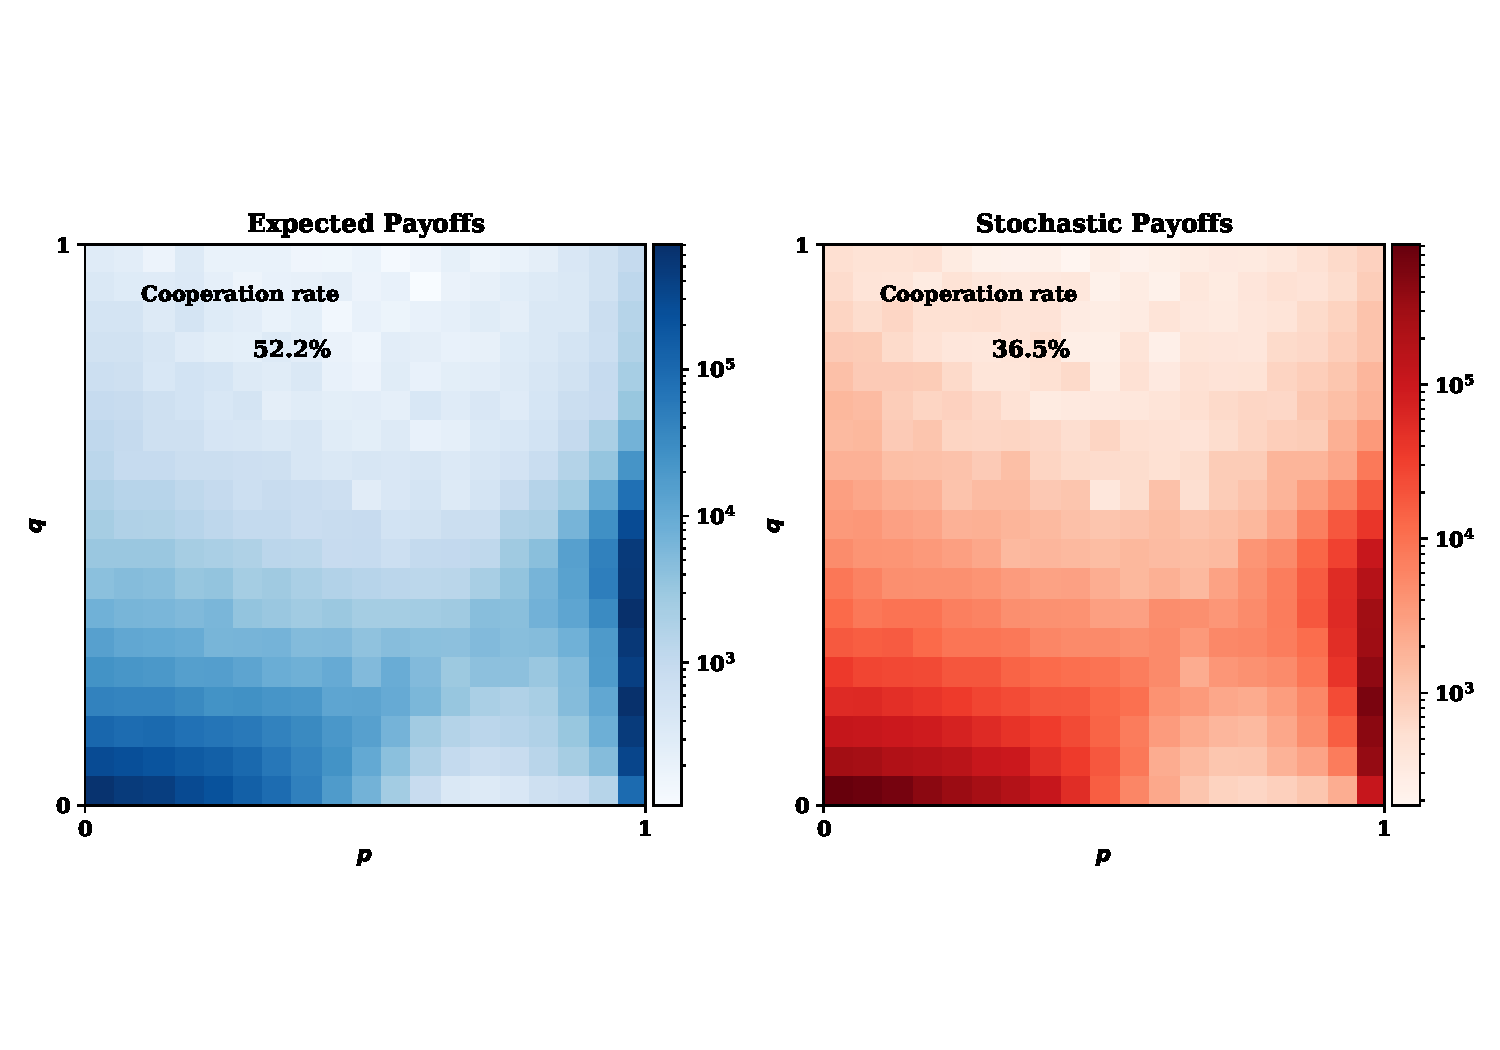
\includegraphics[width=.70\textwidth]{static/expected_and_stochastic_for_donation_game.pdf}
    % 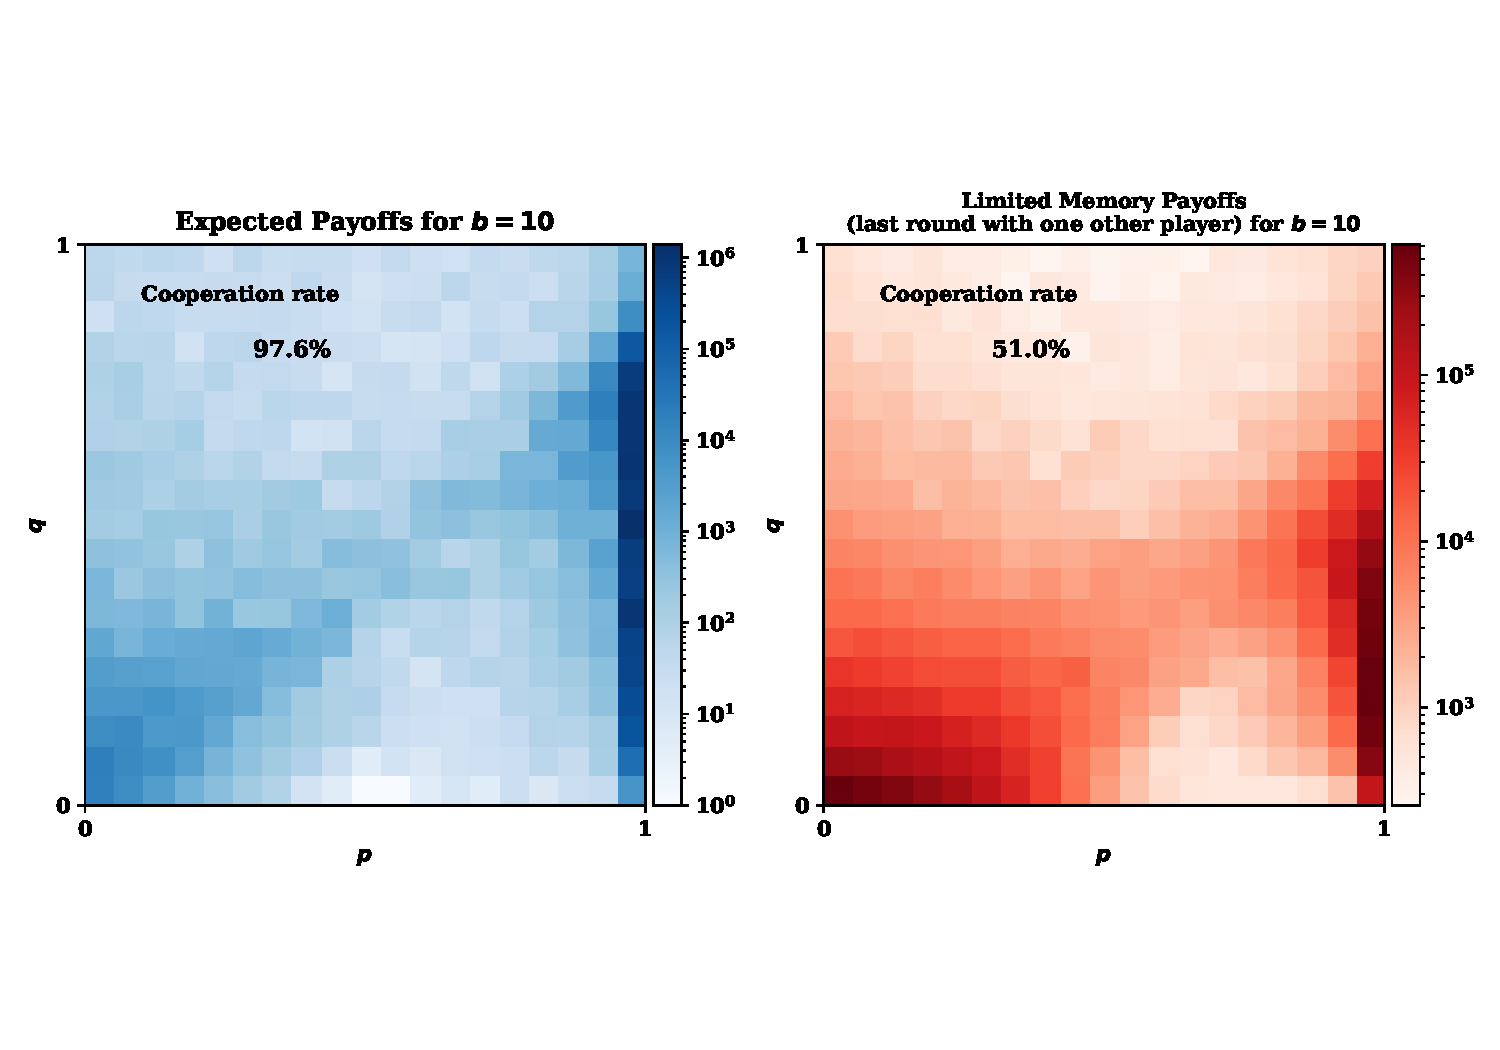
\includegraphics[width=.70\textwidth]{static/expected_and_stochastic_for_donation_game_b_10.pdf}
    \caption{{\bf Evolutionary dynamics under expected payoffs and last round with one interaction payoffs.} 
    We have run two simulations of the evolutionary process described in
    section~\ref{section:model} for $t\!=\!10^7$ time steps. For each time step,
    we have recorded the current resident population ($y,p,q$). Since
    simulations are run for a relatively high continuation probability of
    $\delta\!=\!0.999$, we do not report the players' initial cooperation
    probability $y$. The graphs show how often the resident population chooses
    each combination ($p,q$) of conditional cooperation probabilities in the
    subsequent rounds. ({\bf A}) If players update based on their expected
    payoffs, the resident population typically applies a strategy for which
    $p\!\approx\!1$ and $q\!\le\!1\!-\!c/b\!=\!0.9$. ({\bf B}) When players
    update their strategies based on their realized payoffs in the last round,
    there are two different predominant behaviors. The resident population
    either consists of defectors (with $p\!\approx\!q\!\approx\!0$) or of
    conditional cooperators. In the latter case, the maximum level of $q$
    consistent with stable cooperation is somewhat smaller compared to the
    expected-payoff setting, $q\!<\!0.5$. The cooperation rate within the
    resident population (averaged over all games and over all time steps) is
    close to 100\%. Parameters: $N\!=\!100$, $c\!=\!1$, $\beta\!=\!1$,
    $\delta\!=\!0.999$.}
    \label{fig:expected_and_stochastic_for_donation}
\end{figure}

\begin{figure}[!htbp]
  \centering
  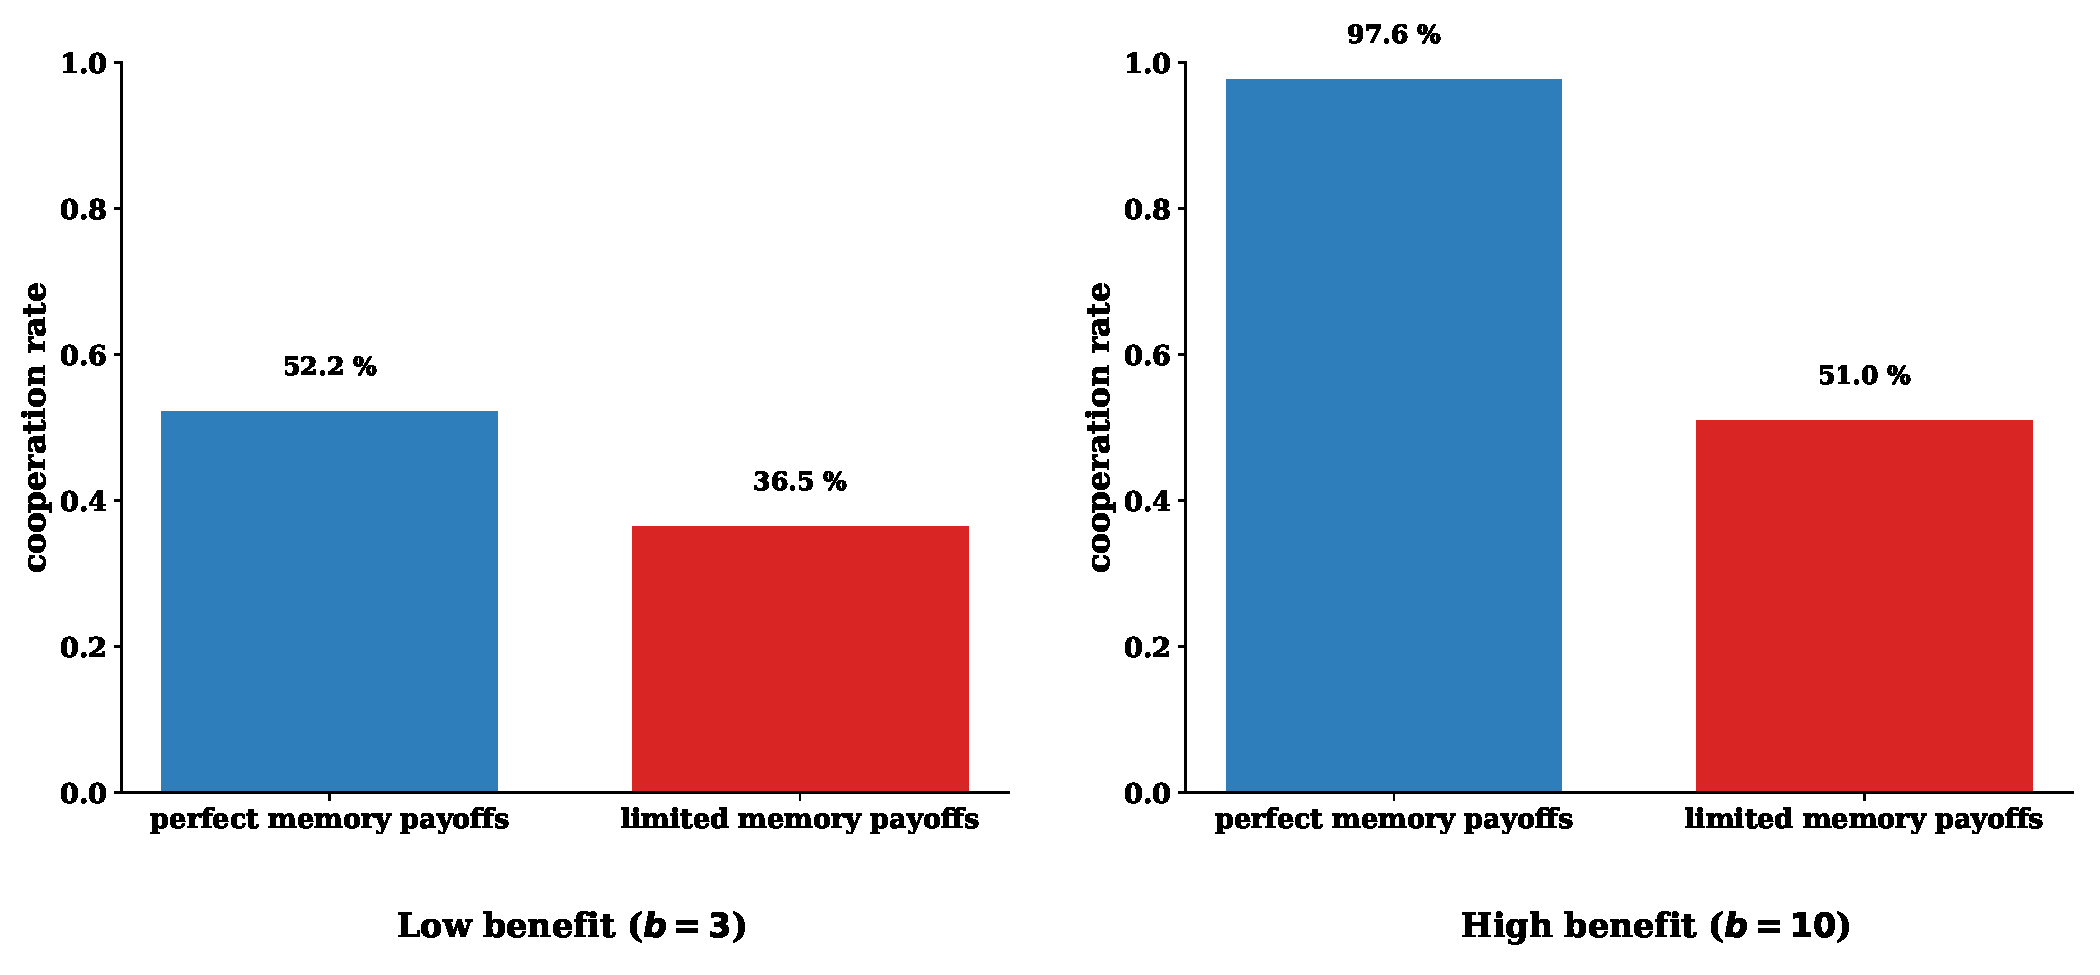
\includegraphics[width=.9\textwidth]{static/cooperation_rates_expected_and_stochastic_for_donation_game.pdf}
\end{figure}

We further explore the effect of benefit in
Figure~\ref{fig:cooperation_rate_over_benefit}. The figure suggests that
expected payoffs always yield a higher cooperation rate. In the case of expected
payoffs we observe that the cooperation rate increases as the value of the
benefit gets higher. In comparison for the limited memory payoffs, the
cooperation rate remains unchanged at approximately 50\% once \(b=5\).

\begin{figure}[!htbp]
  \centering
  \begin{subfigure}{.5\textwidth}
    \centering
    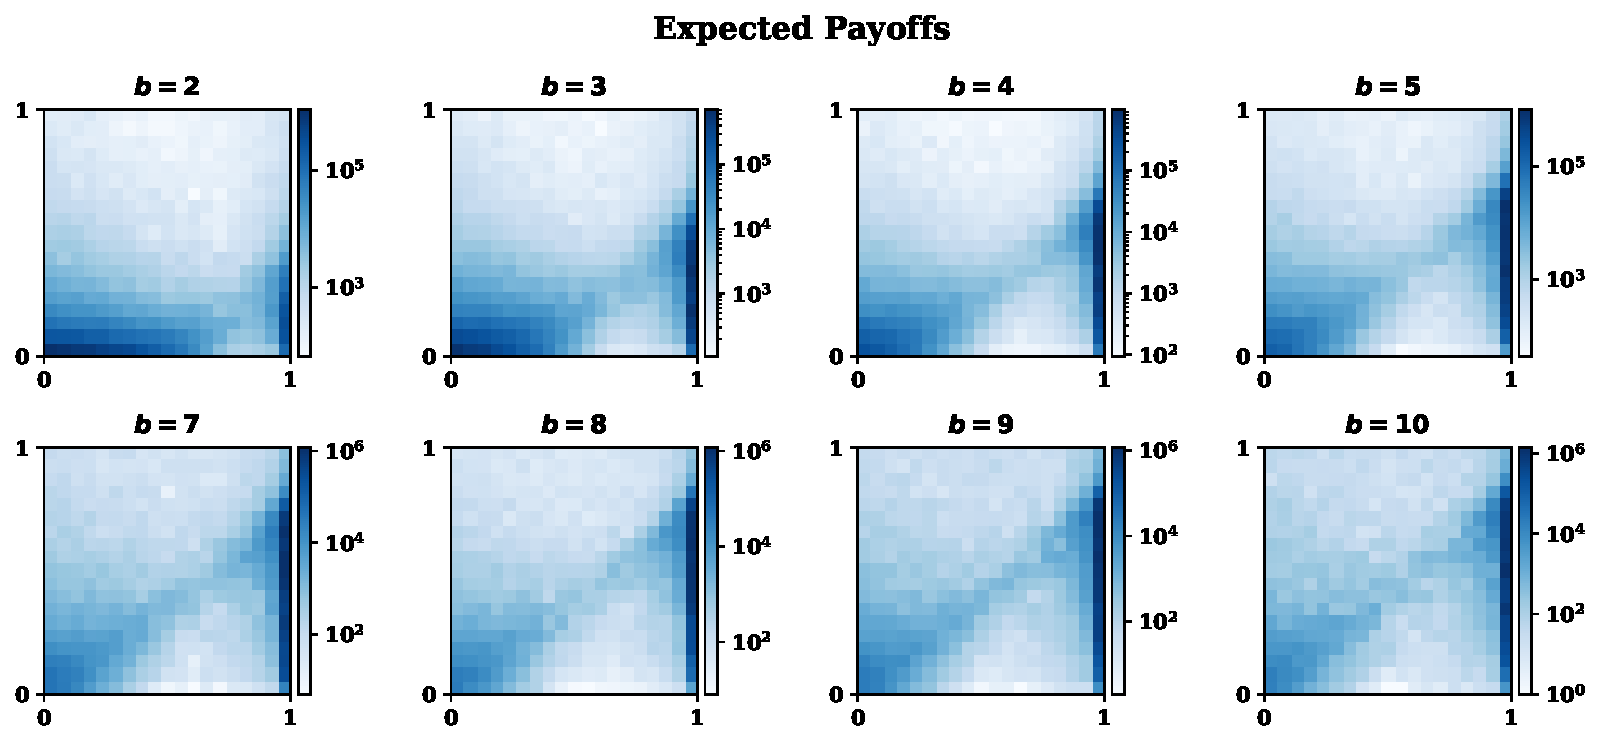
\includegraphics[width=\textwidth]{static/expected_for_beta.pdf}
    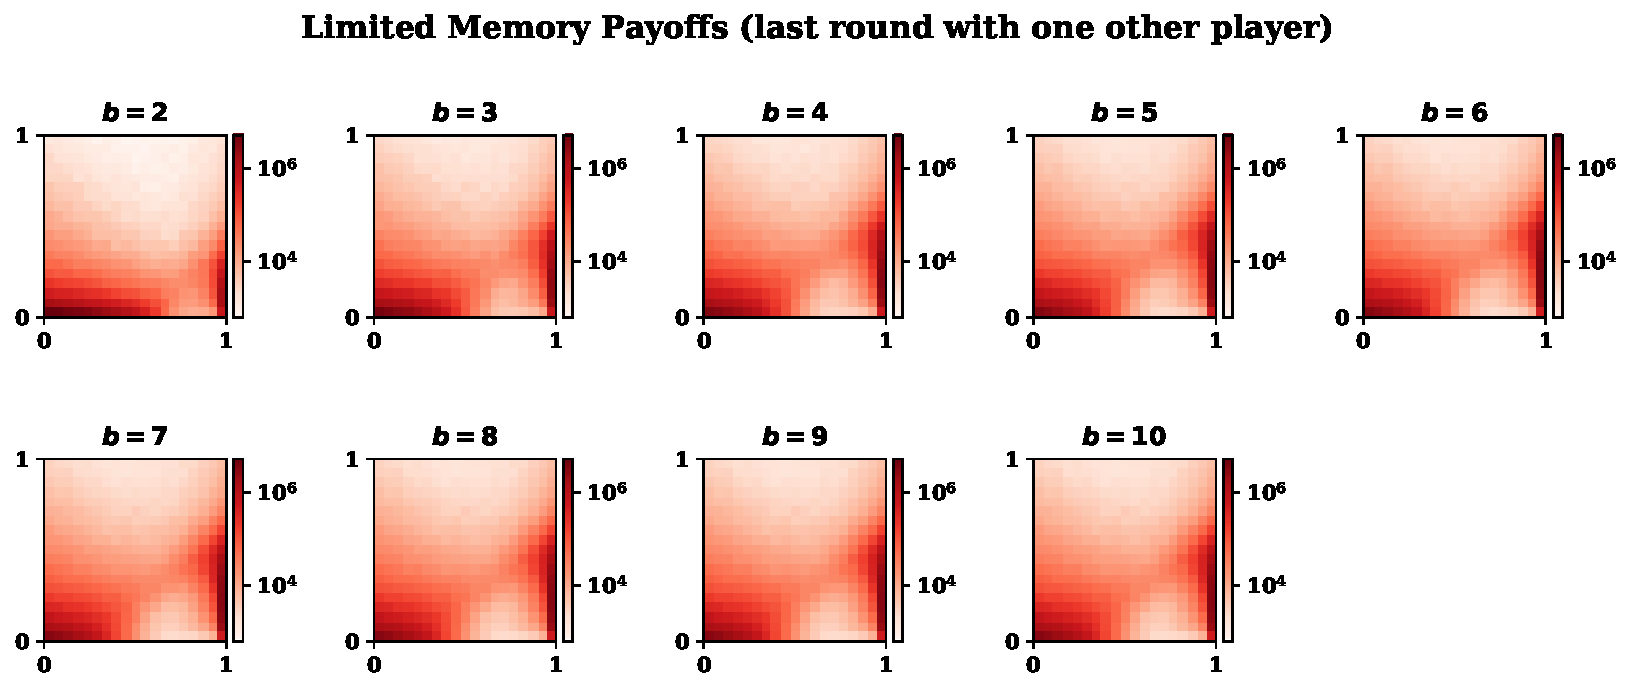
\includegraphics[width=\textwidth]{static/stochastic_for_beta.pdf}
  \end{subfigure}%
  \begin{subfigure}{.5\textwidth}
    \centering
    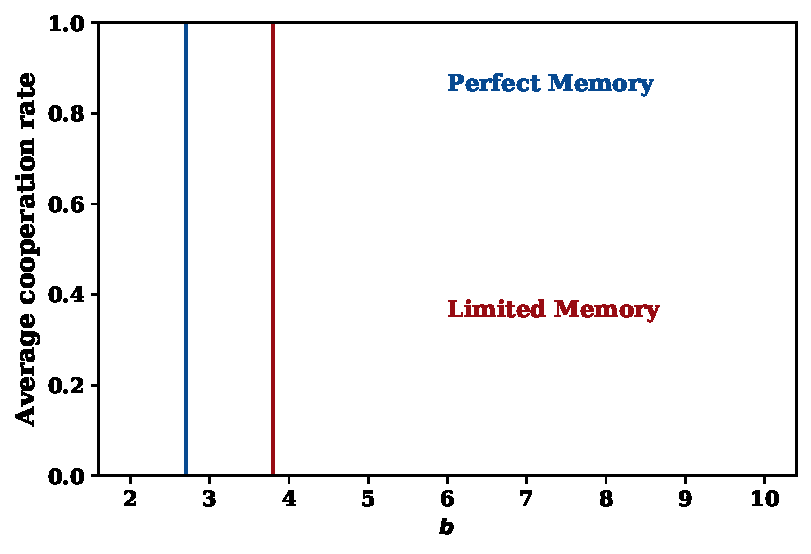
\includegraphics[width=\textwidth]{static/cooperation_rate_over_b.pdf}
  \end{subfigure}
  \caption{{\bf The evolution of cooperation for different benefit values.} 
  We vary the benefit of defection $b$. In all cases, expected payoffs appear to
  overestimate the average cooperation rate the population achieves. ({\bf A})
  the probabilities \(p, q\) for resident population over \(10^7\) time steps
  for each benefit value. ({\bf B}) The cooperation rate within the resident
  population (averaged over all games and over all time steps) over the benefit.
  Unless explicitly varied, the parameters of the simulation are $N\!=\!100$,
  $c\!=\!1$, $\beta\!=\!1$, $\delta\!=\!0.99$. Simulations are run for
  $t\!=\!5\times 10^7$ time steps for each parameter
  combination.}\label{fig:cooperation_rate_over_benefit}
\end{figure}

We also investigate the effect of the strength of selection $\beta$.
Figure~\ref{fig:cooperation_rate_over_betas} illustrates results for various
runs of the evolutionary process. For weak selection, \(\beta < 1\), we observe
that the two methods yield similar results, however, as \(\beta\) increases
there is variation in the evolving populations. In the case of expected payoffs
the resident populations become more cooperative as \(\beta\) increases, whereas
in the case of limited memory payoffs, the resident populations become more
defective.

\begin{figure}[!htbp]
  \centering
  \begin{subfigure}{.65\textwidth}
    \centering
    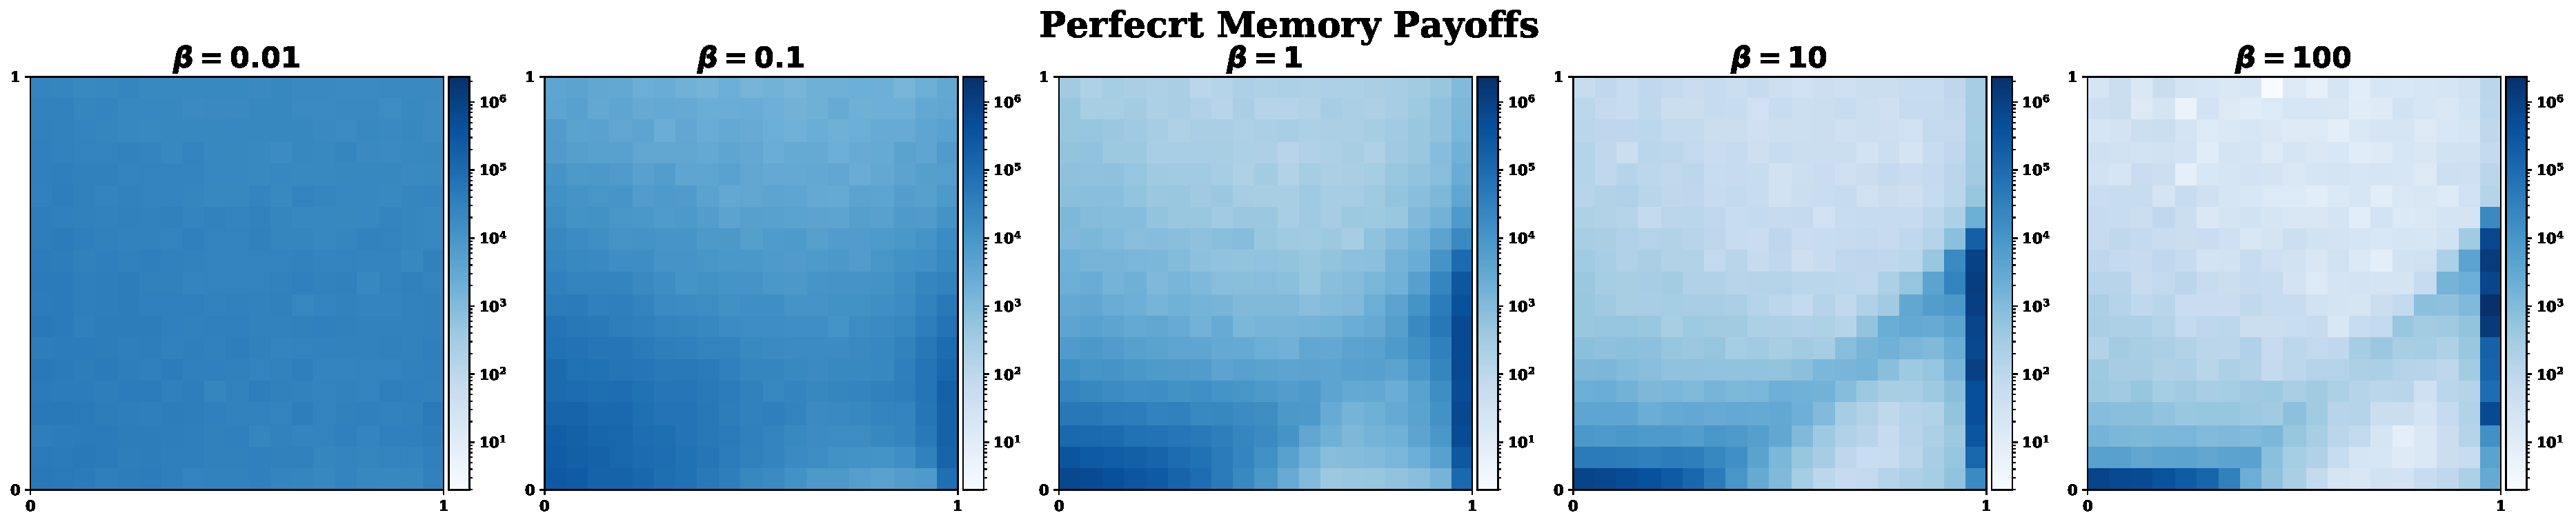
\includegraphics[width=\textwidth]{static/expected_for_selection_strenght.pdf}
    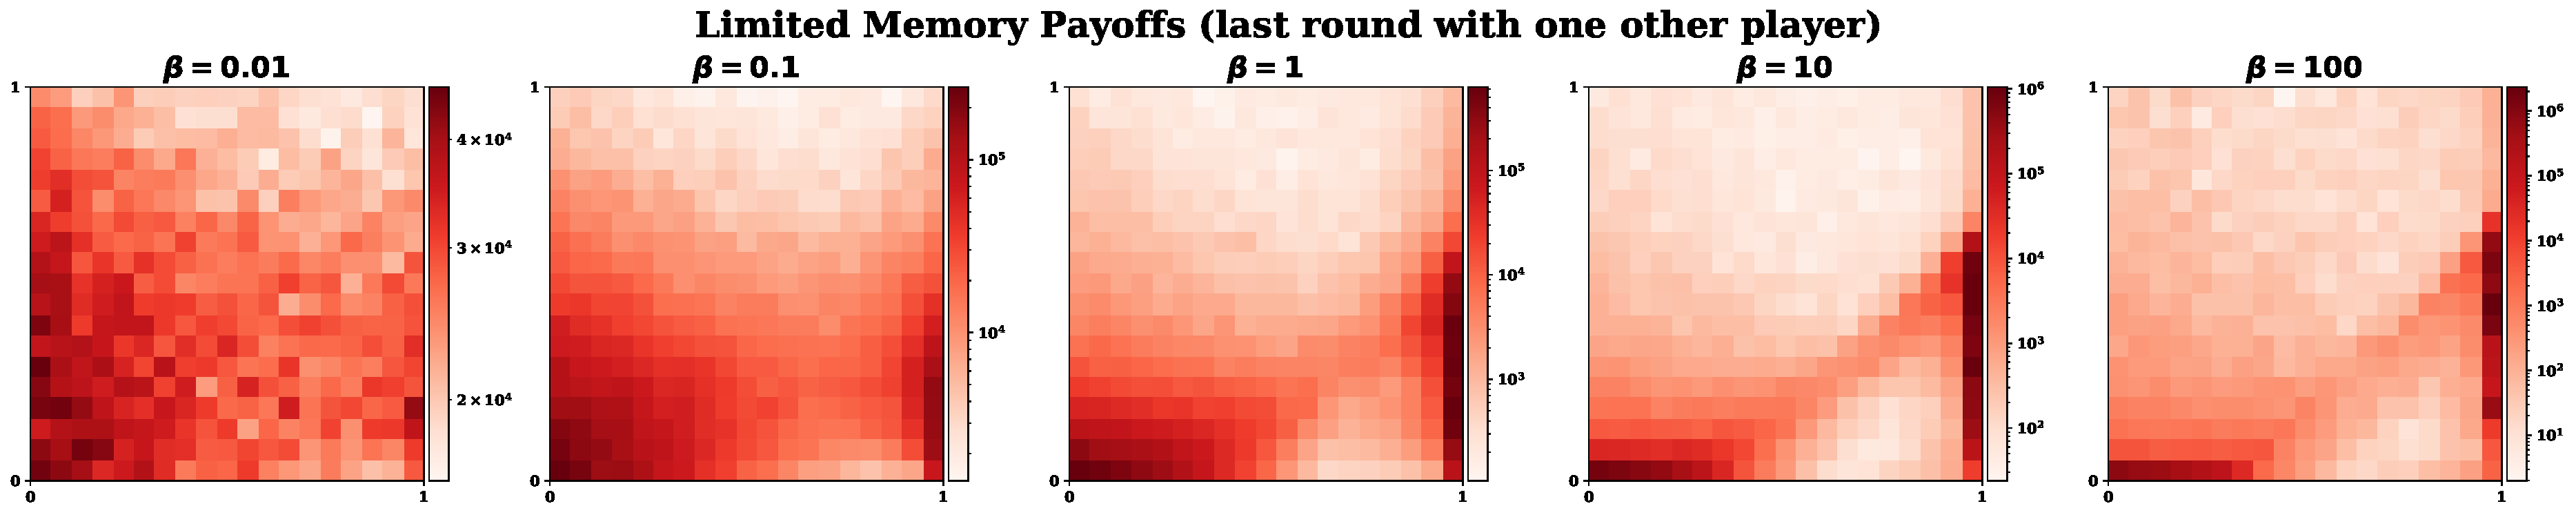
\includegraphics[width=\textwidth]{static/stochastic_for_selection_strenght.pdf}
  \end{subfigure}%
  \begin{subfigure}{.35\textwidth}
    \vspace{.3cm}
    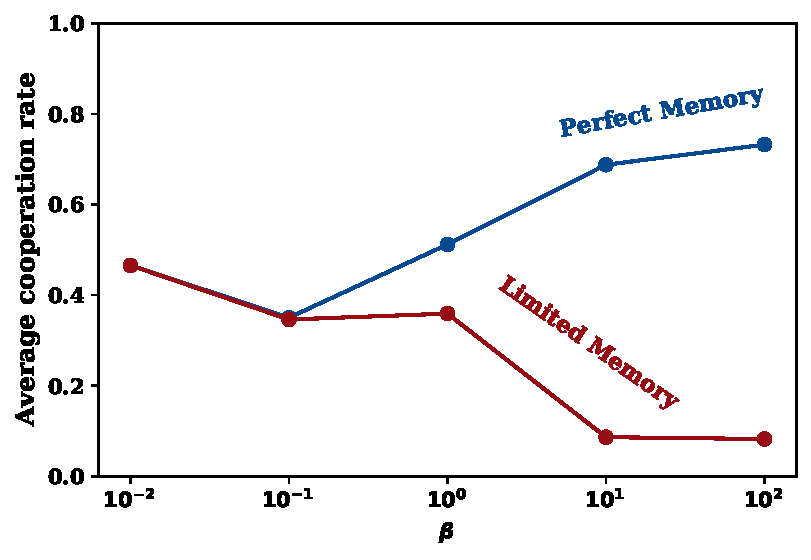
\includegraphics[width=\textwidth]{static/cooperation_rate_over_betas.pdf}
  \end{subfigure}
\caption{{\bf The evolution of cooperation for different selection strength values.}
We vary the selection strength $\beta$. In all cases, stochastic payoff
evaluation tends to reduce the evolving cooperation rates. ({\bf A}) the
probabilities \(p, q\) for resident population over \(10^7\) time steps for each
\(\beta\) value. ({\bf B}) The cooperation rate within the resident population
(averaged over all games and over all time steps) over \(\beta\). Unless
explicitly varied, the parameters of the simulation are $N\!=\!100$, $b\!=\!3$,
$c\!=\!1$, $\beta\!=\!1$, $\delta\!=\!0.99$. Simulations are run for
$t\!=\!5\times 10^7$ time steps for each parameter
combination.}\label{fig:cooperation_rate_over_betas}
\end{figure}

% \subsection{Effect of updating payoffs in different social
% dilemmas}\label{section:2_by_2_games}

% In the previous section we gained insights into the effects of the updating
% payoffs, and into how parameters such as the benefit and the strength of
% selection can intensify them. We investigated these effects by using the
% donation game. In order to broaden our understanding of the updating payoffs on
% different forms of possible human interactions we extend our approach to all \(2
% \times 2\) symmetric games. More specifically, we apply our analysis to four
% different classes of games; the harmony, the snowdrift, the prisoner's dilemma
% and the stag-hunt games.

% We compare the results of the evolutionary process when the updating payoffs are
% based on the expected payoffs, and on the last round payoffs for all the four
% possible classes of games (Figures~\ref{fig:expected_two_by_two}
% and~\ref{fig:last_round_two_by_two}). In Figure~\ref{fig:expected_two_by_two}
% each sub figure represents a run of evolutionary process for a different set of
% values for \(\mathcal{U}\). Without loss of generality we set \(R=1\) and
% \(P=0\)~\cite{Martinez2012, Roca2009}, and we vary the values of the temptation
% payoff \(T\) (across the \(x\)-axis) and of the sucker's payoff \(S\) (across
% the \(y\)-axis). Starting at the upper left corner and proceeding clockwise the
% quadrants correspond to the harmony, the snowdrift, the prisoner's dilemma and
% the stag-hunt games.

% \begin{figure}[!htbp]
%   \centering
%   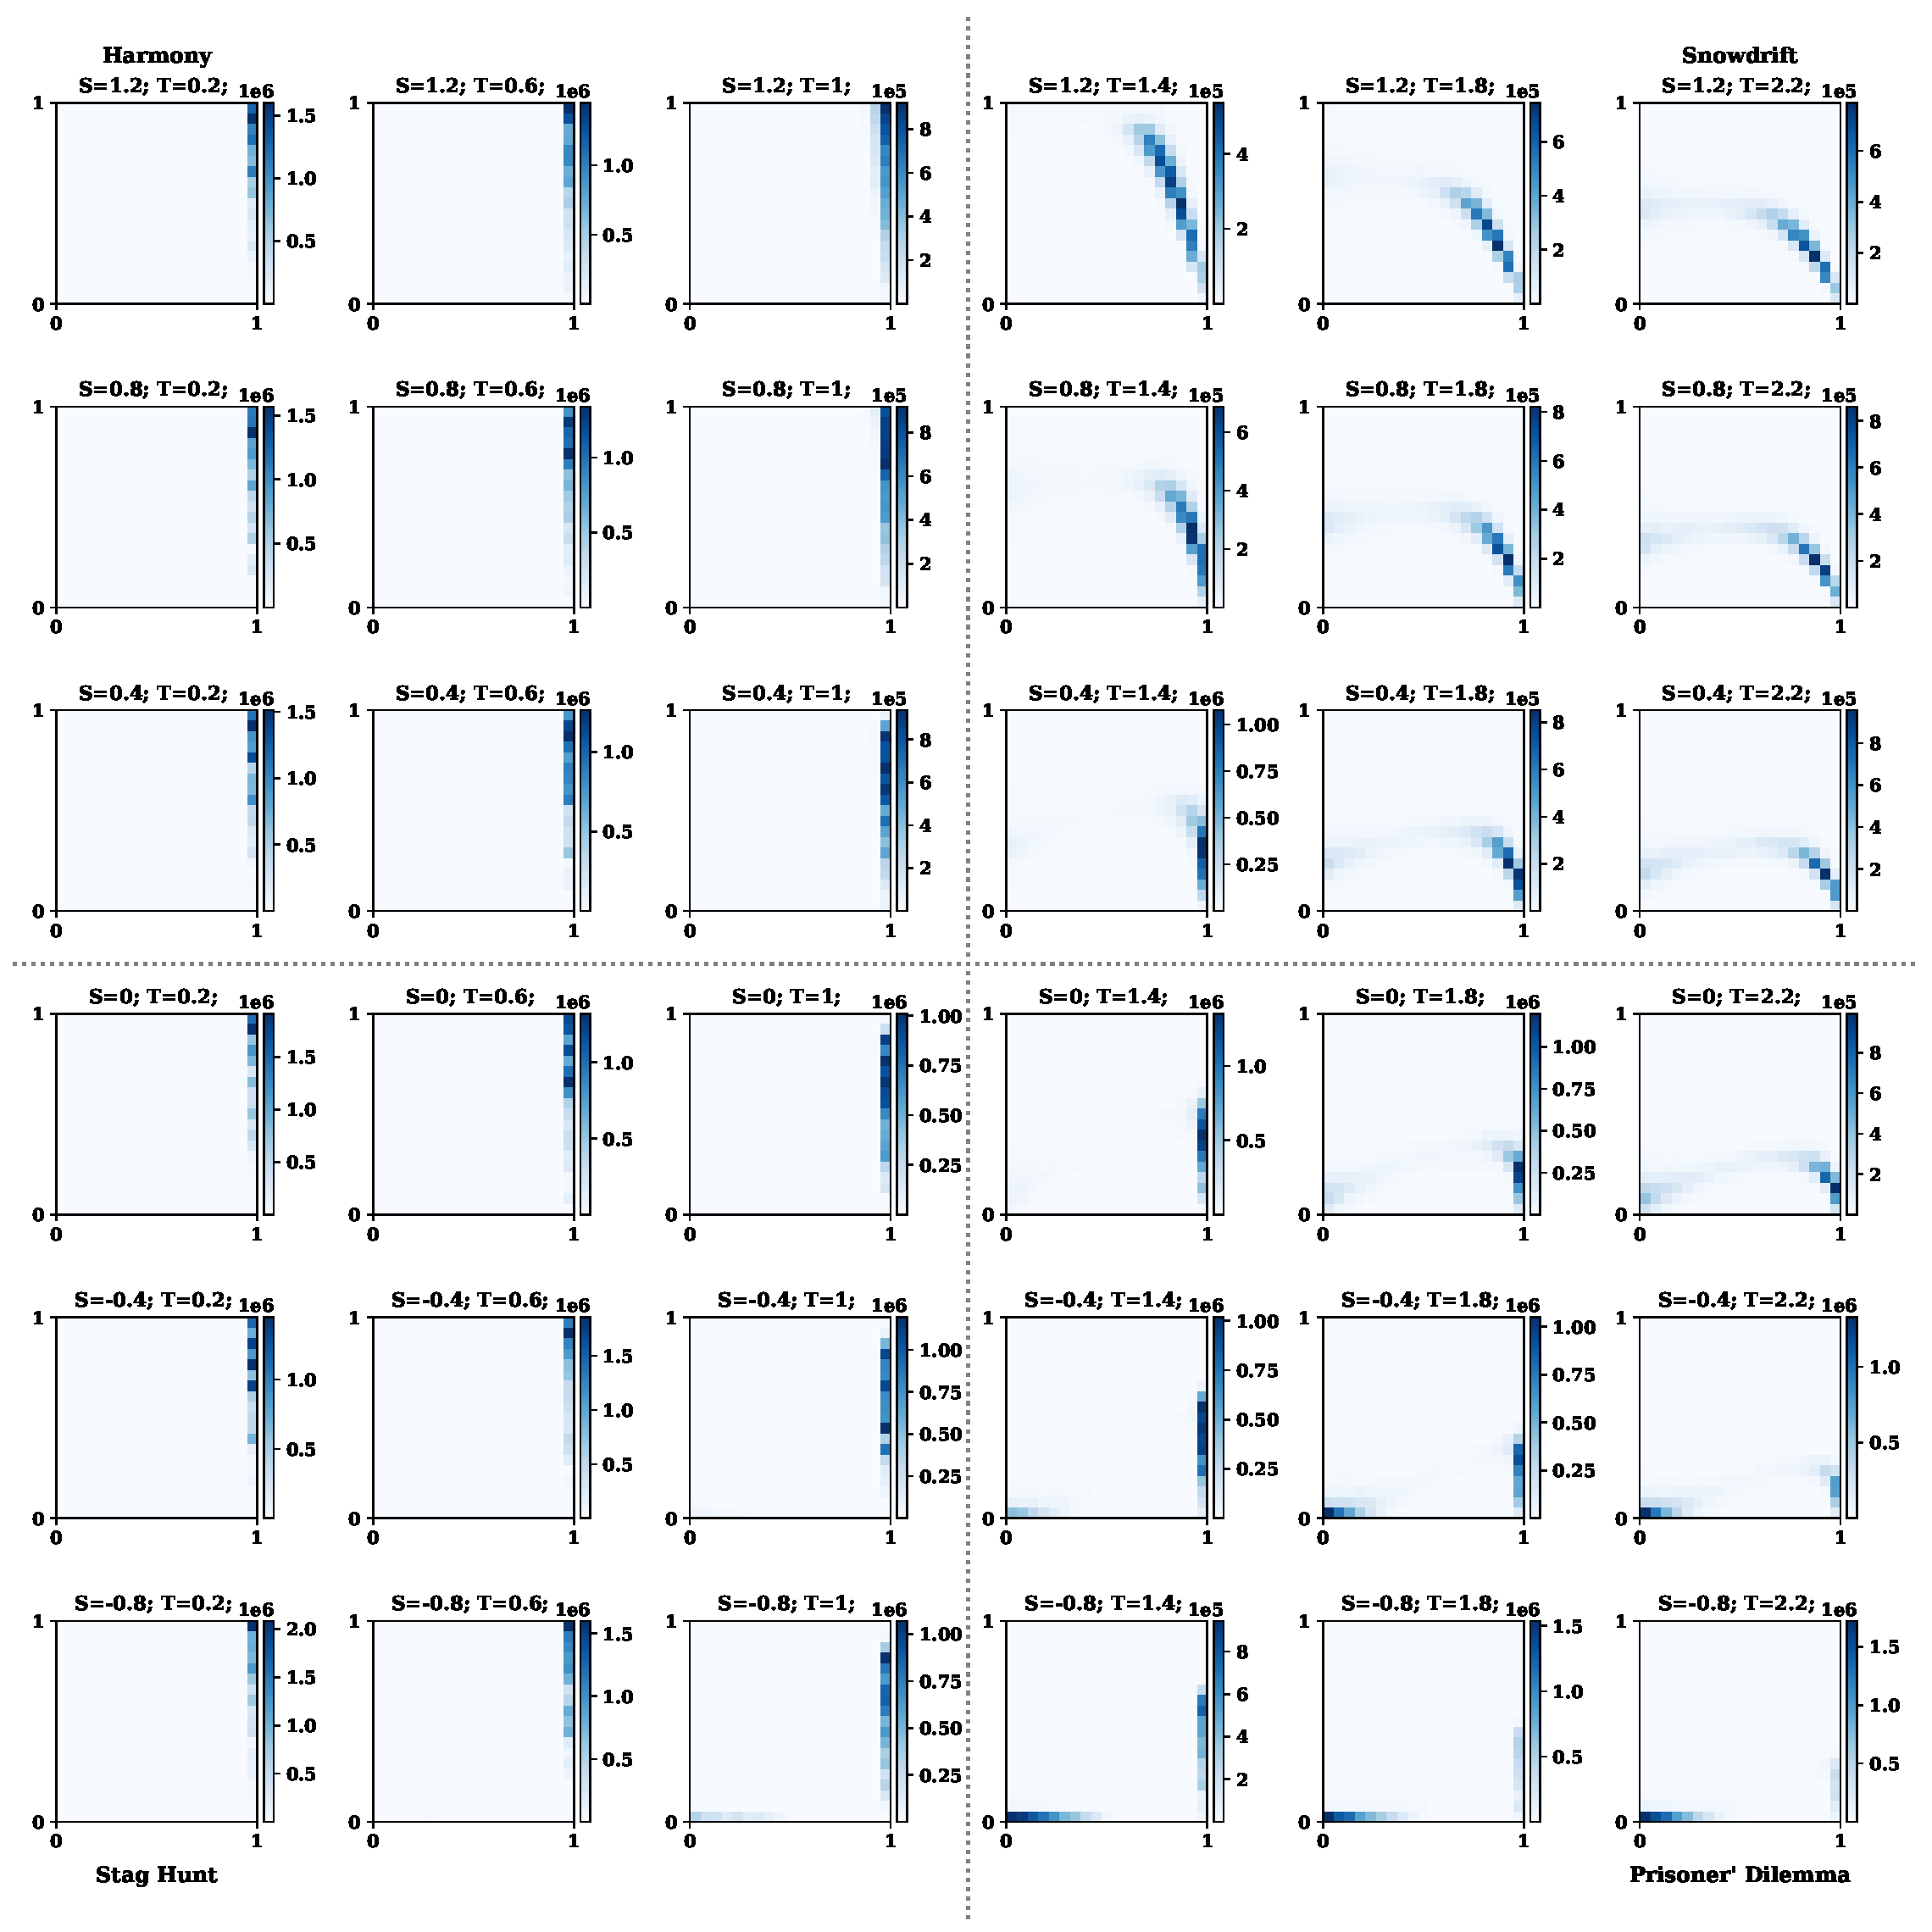
\includegraphics[width=\textwidth]{static/expected_two_by_two_games.pdf}
%   \caption{{\bf Evolutionary dynamics under expected payoffs for various social dilemmas.}
%   We vary the temptation payoff \(T \in \{0.2, 0.6, 1, 1.4, 1.8, 2.2\}\) across
%   the \(x\) axis, and  \(S \in \{1.2, 0.8, 0.4, 0, -0.4, -0.8\}\) across the
%   \(y\) axis. ({\bf A}) The top left quadrant where \(S > 0\) and \(T \leq 1\)
%   corresponds to the harmony game. The preference ordering for the harmony game
%   is \(R > T > S > P\). ({\bf B}) The top right quadrant where \(S > 0\) and \(T
%   > 1\) corresponds to the snowdrift game. The preference ordering for the
%   snowdrift game is \(T > R > S > P\). ({\bf C}) The bottom left quadrant where
%   \(S < 0\) and \(T \leq 1\) corresponds to the stag-hunt game. The preference
%   ordering for the stag-hunt game is \(R > T > P > S\). ({\bf D}) The bottom
%   right quadrant where \(S < 0\) and \(T > 1\) corresponds to the prisoner's
%   dilemma game. The preference ordering for the prisoner's dilemma game is \(T >
%   R > P > S\). Unless explicitly varied, the parameters of the simulation are
%   $N\!=\!100$, $\beta\!=\!10$, $\delta\!=\!0.99$, $t\!=\!5\times 10^7$.}
%   \label{fig:expected_two_by_two}
% \end{figure}


% \begin{figure}[!htbp]
%   \centering
%   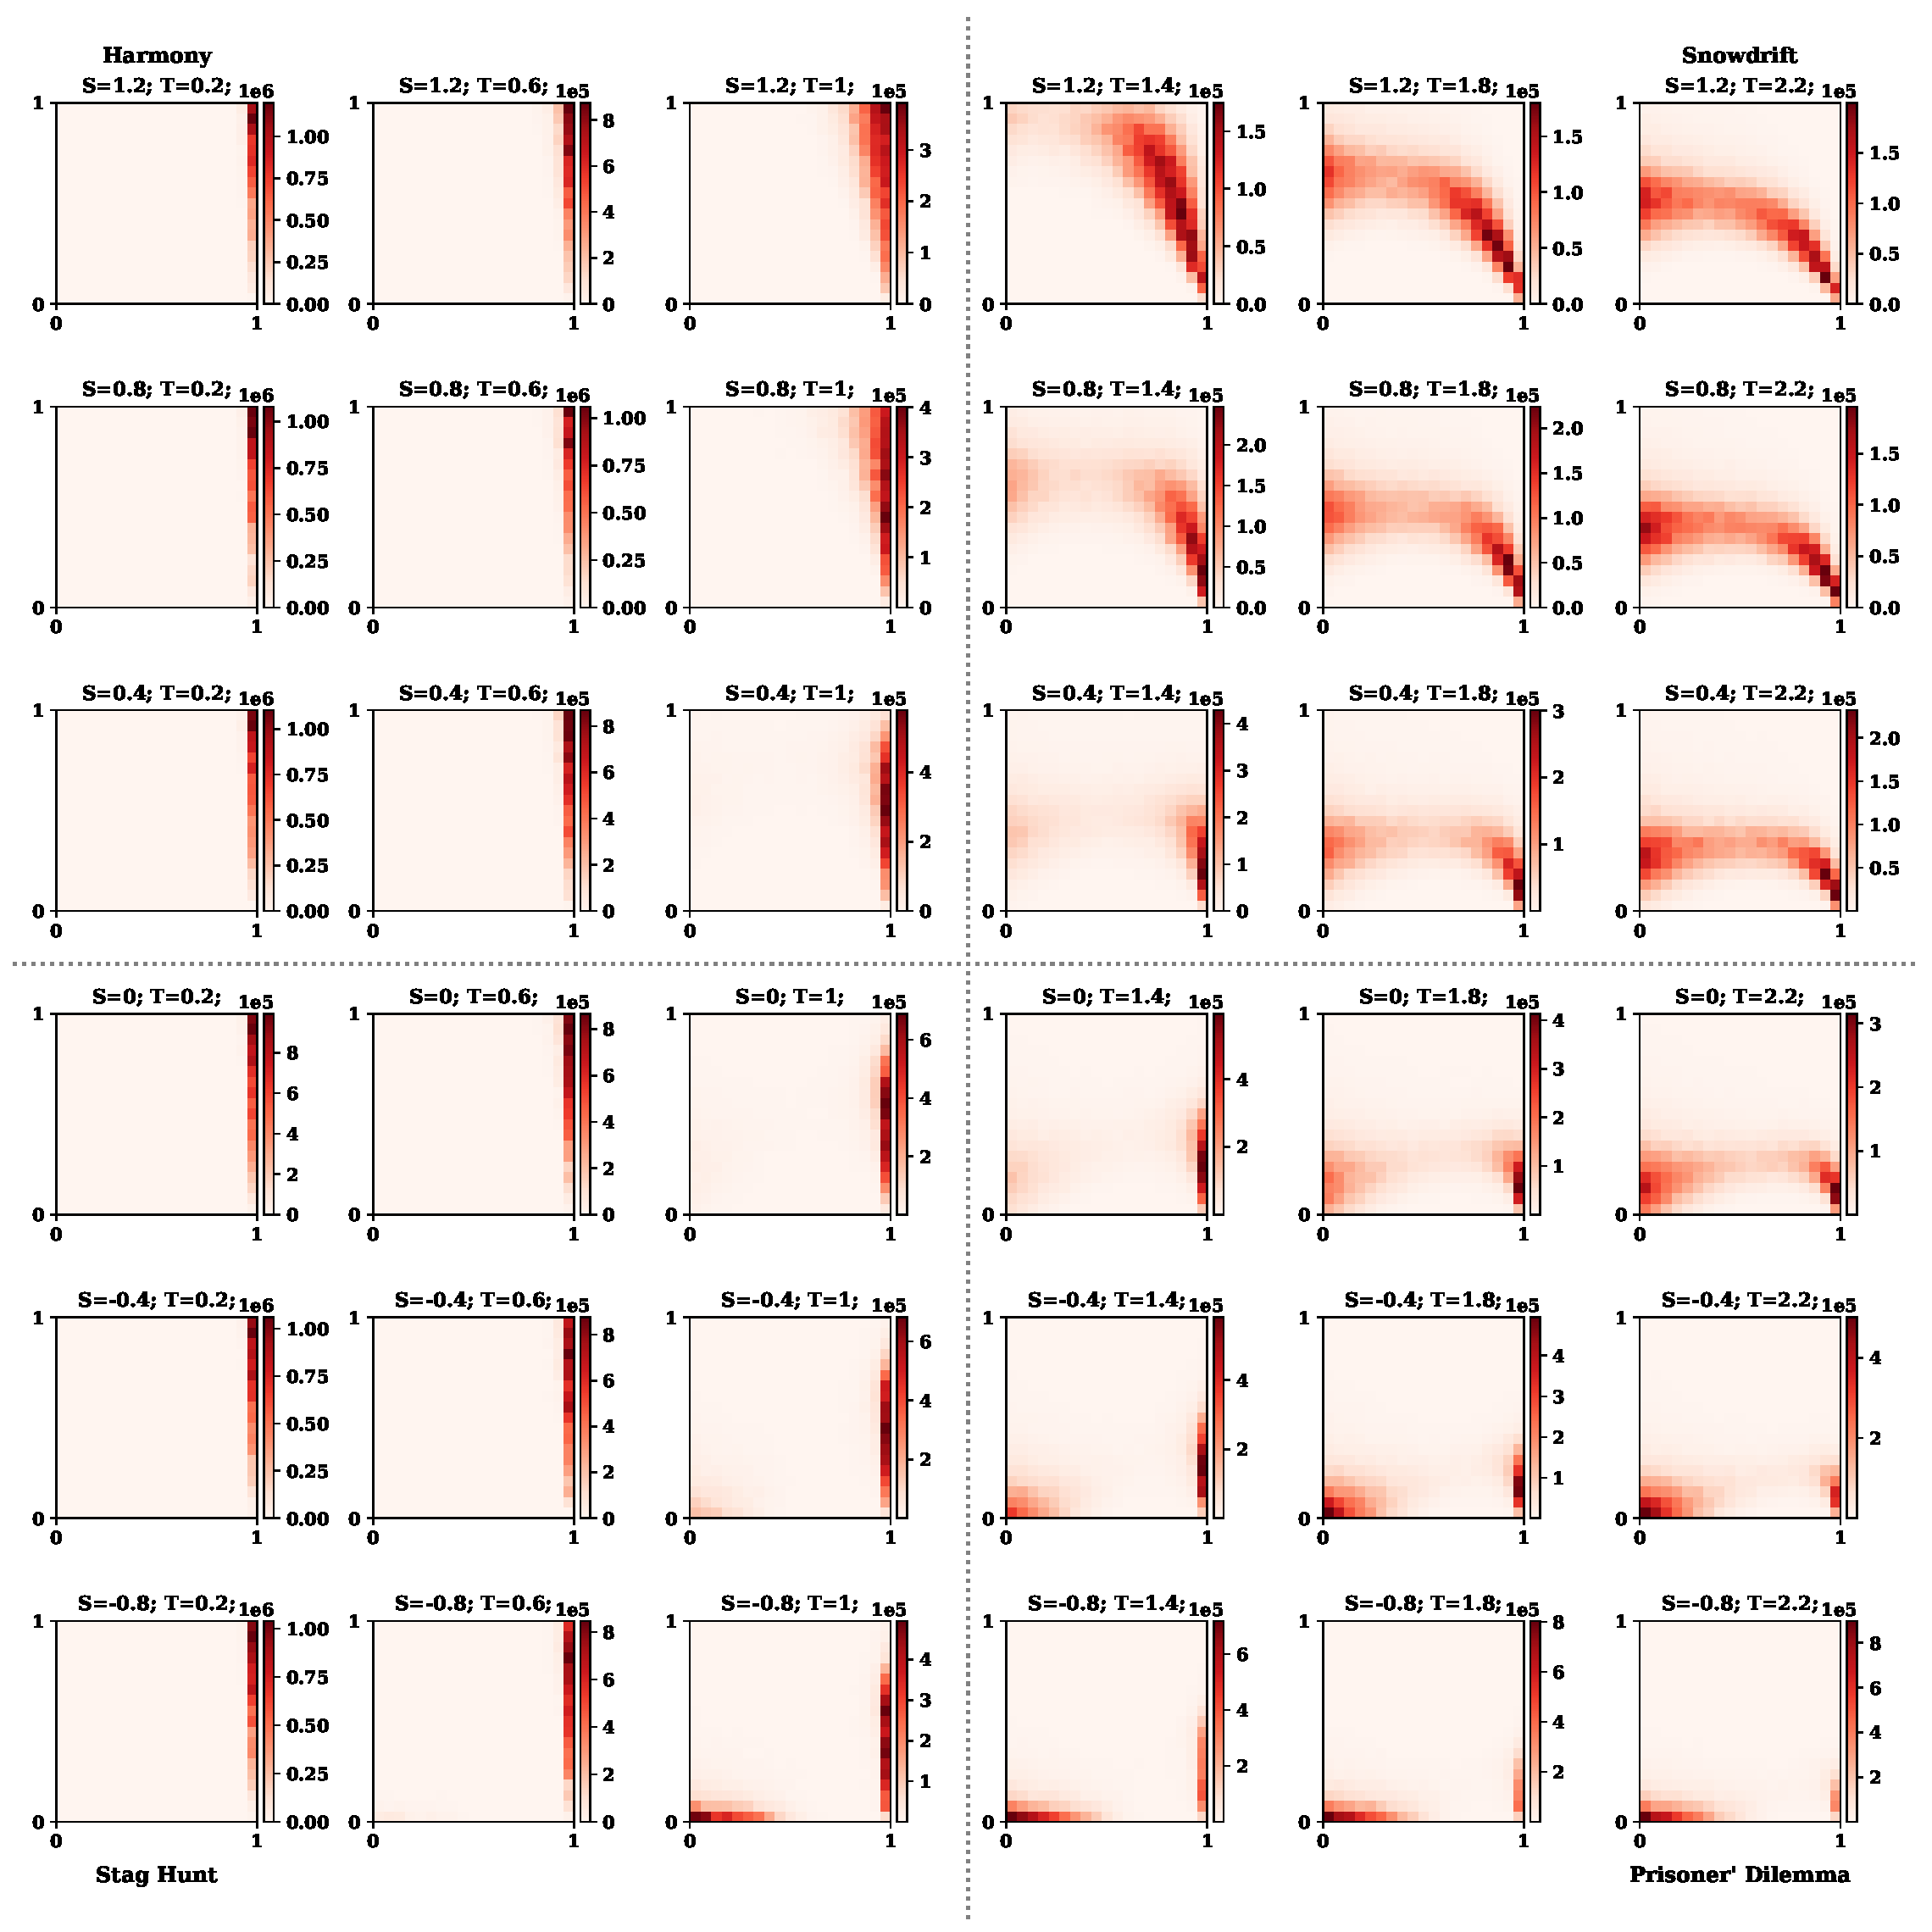
\includegraphics[width=\textwidth]{static/stochastic_two_by_two_games.pdf}
%   \caption{{\bf Evolutionary dynamics under last round payoffs for various social dilemmas.} 
%   We vary the temptation payoff \(T \in \{0.2, 0.6, 1, 1.4, 1.8, 2.2\}\) across
%   the \(x\) axis, and  \(S \in \{1.2, 0.8, 0.4, 0, -0.4, -0.8\}\) across the
%   \(y\) axis. ({\bf A}) The top left quadrant where \(S > 0\) and \(T \leq 1\)
%   corresponds to the harmony game. The preference ordering for the harmony game
%   is \(R > T > S > P\). ({\bf B}) The top right quadrant where \(S > 0\) and \(T
%   > 1\) corresponds to the snowdrift game. The preference ordering for the
%   snowdrift game is \(T > R > S > P\). ({\bf C}) The bottom left quadrant where
%   \(S < 0\) and \(T \leq 1\) corresponds to the stag-hunt game. The preference
%   ordering for the stag-hunt game is \(R > T > P > S\). ({\bf D}) The bottom
%   right quadrant where \(S < 0\) and \(T > 1\) corresponds to the prisoner's
%   dilemma game. The preference ordering for the prisoner's dilemma game is \(T >
%   R > P > S\). Unless explicitly varied, the parameters of the simulation are
%   $N\!=\!100$, $\beta\!=\!10$, $\delta\!=\!0.99$, $t\!=\!5\times 10^7$.}
%   \label{fig:last_round_two_by_two}
% \end{figure}

% The harmony game describes an interaction without conflict. In the harmony game
% it is in the best interest for both players to cooperate, and in an evolutionary
% process cooperators prevail. We observe that for most harmony game runs the
% resident population overwhelmingly applies a strategy for which \(p\) and \(q\)
% are \(\approx 1\) (Figure~\ref{fig:expected_two_by_two}). The snowdrift game
% describes a situation similar to that of the prisoner's dilemma; cooperation
% results in a benefit to the opposing player but entailing a cost to the
% cooperator. However, in the snowdrift game individuals obtain immediate direct
% benefits from the cooperative acts which leads to \(S > P\). In the snowdrift
% game more cooperation emerges compared to the prisoner's dilemma. Defection is
% never a resident strategy and for the same values of temptation the overall
% \(q-\) values are higher. The last class of games we present are for the
% stag-hunt game. In the stag-hunt game there is an equilibrium in which both
% players cooperate as well as one in which both defect. For small values of the
% temptation and the sucker's payoffs we observe that cooperation prevails similar
% to the harmony game. However, in the case where the temptation and the reward
% payoffs are equal the resident population either consists of defectors or
% cooperators.

% Although the patterns of the evolved populations remain similar if we consider
% that players update their strategies based on their last round payoff
% (Figure~\ref{fig:last_round_two_by_two}), there are still dissimilarities
% between the two approaches. To better understand these dissimilarities, we
% explore the cooperation rates for each of the cases of the social dilemmas we
% have presented (Figure~\ref{fig:cooperation_rates_two_by_two_part_one}).

% In the harmony game the cooperation rates for both approaches are similar. The
% biggest difference occurs for \(T=1\), nevertheless, it is less than 10\%. There
% are two instances for which the cooperation rates are higher for the limited
% memory payoffs compared to the expected. These are for \(T=2.2, S=0.4\) and for
% \(T=2.2, S=0.8\). It is only in the snowdrift game that cooperation is
% overestimated when a minimum of information is considered. Players are slightly
% more likely to cooperate after a cooperation and to forgive after being at the
% receiving end of a defection. For the rest of the cases the classical scenario
% overestimates the average cooperation rate, supporting the results of the
% previous section. There is a substantial difference in the cooperation rates for
% the prisoner's dilemma class. We observe that for \(S<-0.4\) cooperation almost
% never emerges if players imitate based only on the last round payoff.

% \begin{figure}[!htbp]
%   \centering
%   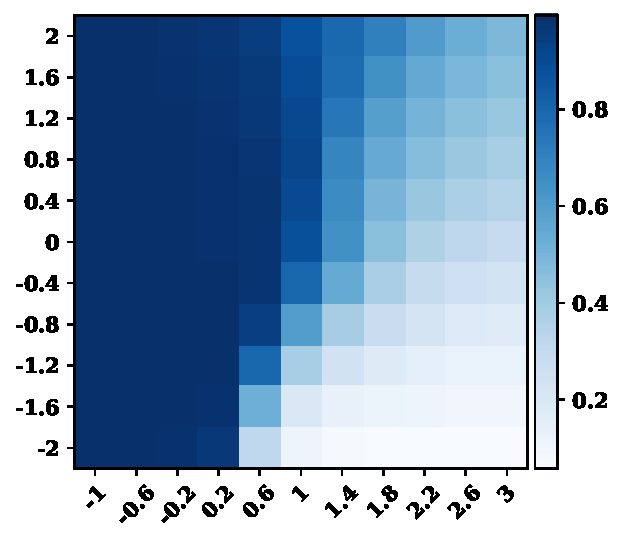
\includegraphics[width=.4\textwidth]{static/expected_two_by_two_games_cooperation.pdf}
%   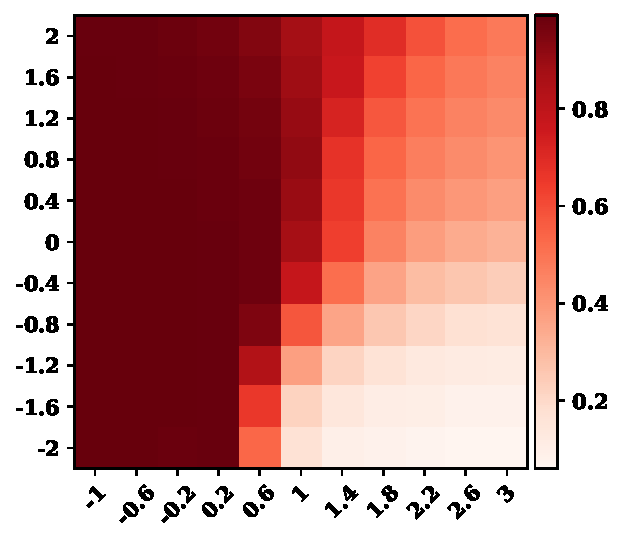
\includegraphics[width=.4\textwidth]{static/stochastic_two_by_two_games_cooperation.pdf}
%   \caption{\textbf{Cooperation rates for various social dilemmas.} ({\bf A}) If
%   players update based on their expected payoffs. ({\bf B}) If players update
%   based on their last round payoffs. We vary the temptation payoff \(T \in
%   \{0.2, 0.6, 1, 1.4, 1.8, 2.2\}\) across the \(x\) axis, and \(S \in \{1.2,
%   0.8, 0.4, 0, -0.4, -0.8\}\) across the \(y\) axis. Unless explicitly varied,
%   the parameters of the simulation are $N\!=\!100$, $\beta\!=\!10$,
%   $\delta\!=\!0.99$, $t\!=\!5\times
%   10^7$.}\label{fig:cooperation_rates_two_by_two_part_one}
% \end{figure}

% So far we have explored the difference between the expected payoffs and the last
% round payoffs. In order to explore further the effect of limited memory we allow
% individuals to remember more. More precisely, up to two interactions and up to
% the last two rounds. In total we present results for three more updating
% payoffs. These are the payoffs when individuals consider the last two rounds
% with another member of the population, the last round with two members of the
% population, and the last two rounds with two members of the population. Similar
% to the last round payoff, we use simulations and record which strategies the
% players adopt over time based
% (Appendix~\ref{appendix:further_simulation_results}) and we compare the evolving
% cooperation rates to those of the expected payoffs
% (Figure~\ref{fig:cooperation_rates_two_by_two_part_two}).

% In the case of the last two rounds payoff we make two observations. Initially,
% for the harmony, the stag-hunt and the prisoner's dilemma classes the average
% cooperation rates are higher than the previous case of the last round payoff.
% The rates remain strictly less than in the expected payoffs, however, in the
% case of the prisoner's dilemma we observe a significant increase. Secondly, for
% the snowdrift class there are more instances for which the cooperation rates are
% higher than in the expected payoffs. This could indicate that in the case of the
% snowdrift game the expected payoffs underestimate cooperation. Once players
% interact with two other members of the population, instead of one, the expected
% payoffs strictly yield a higher cooperation rate  even in the case of the
% snowdrift game. Similar to the previous result, the difference between the two
% approaches is always higher for the prisoner's dilemma class.

% \begin{figure}[!htbp]
%   \centering
%   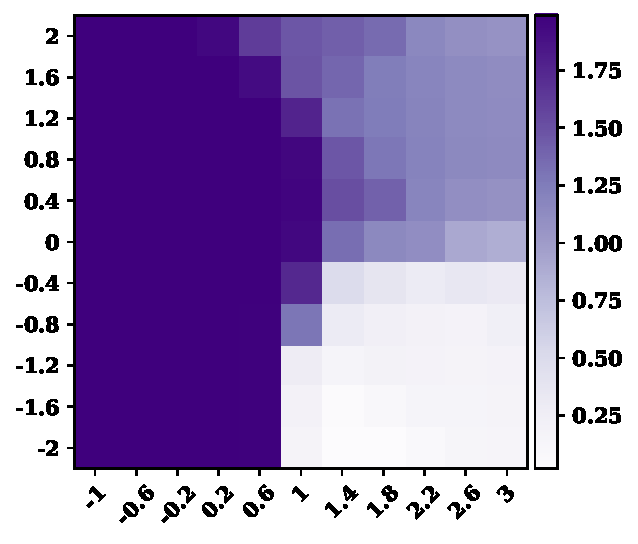
\includegraphics[width=.33\textwidth]{static/rounds_two_by_two_games_cooperation.pdf}
%   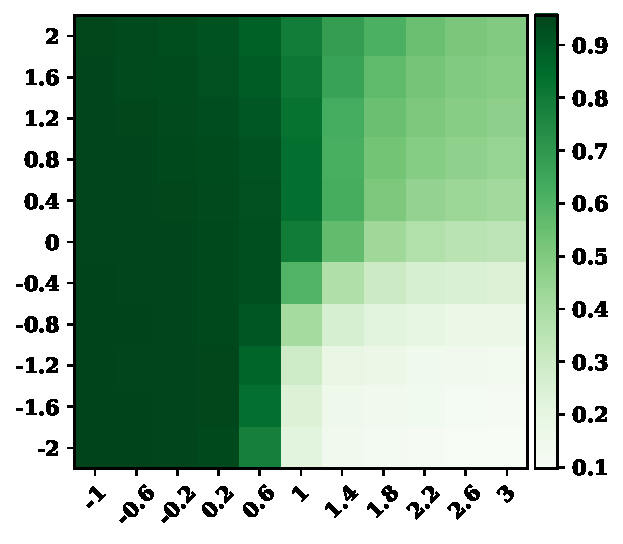
\includegraphics[width=.33\textwidth]{static/opponents_two_by_two_games_cooperation.pdf}
%   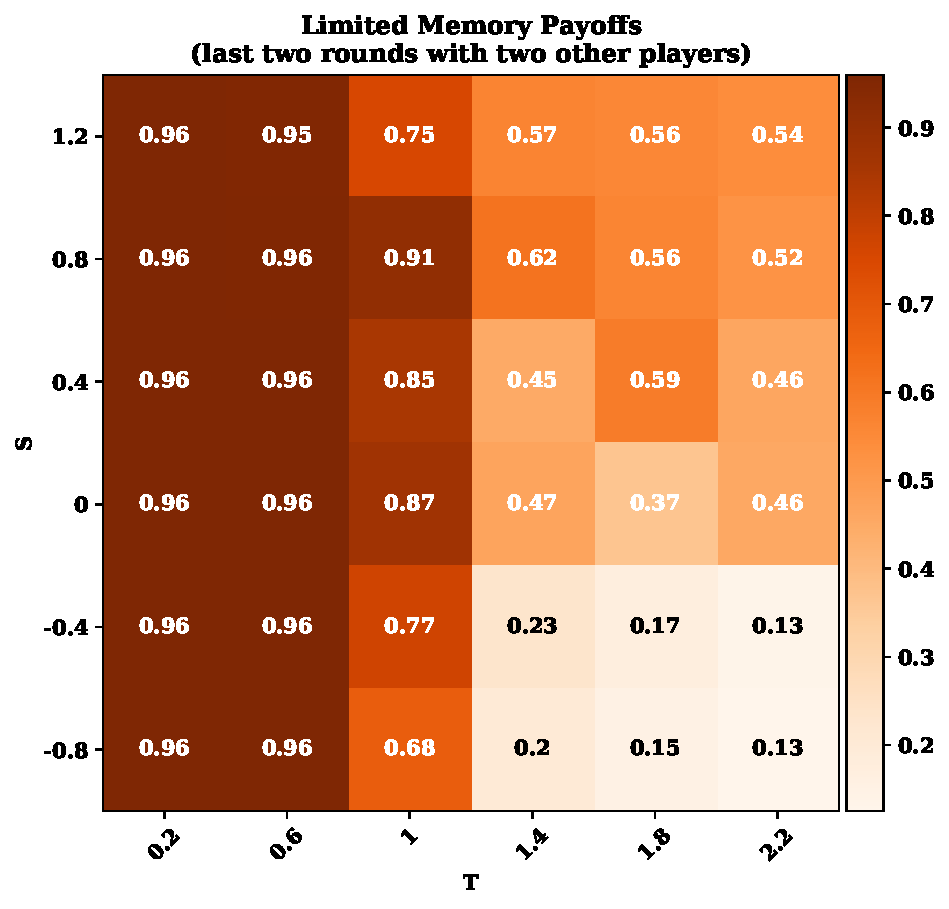
\includegraphics[width=.33\textwidth]{static/rounds_opponents_two_by_two_games_cooperation.pdf}
%   \caption{\textbf{Cooperation rates over various social dilemmas for different
%   limited memory payoffs.} ({\bf A}) If players update based on their last two
%   rounds with another member of the population. ({\bf B}) If players update
%   based on their last round with two other members of the population. ({\bf C})
%   If players update based on their last two rounds with two other members of the
%   population. We vary the temptation payoff \(T \in \{0.2, 0.6, 1, 1.4, 1.8,
%   2.2\}\) across the \(x\) axis, and \(S \in \{1.2, 0.8, 0.4, 0, -0.4, -0.8\}\)
%   across the \(y\) axis. Unless explicitly varied, the parameters of the
%   simulation are $N\!=\!100$, $\beta\!=\!10$, $\delta\!=\!0.99$, $t\!=\!5\times
%   10^7$..}
%   \label{fig:cooperation_rates_two_by_two_part_two}
% \end{figure}


\section{Conclusions}\label{section:conclusions}

Cooperation can be seen at odd, why is it that we choose to help others,
increasing their payoff, at the expense of decreasing one's own? In spite of all
the selfish genes’ animal and human communities seem to altruistically help each
other and cooperate, and evolutionary game theory has helped us shape our
understanding of the evolution of cooperation.

Previous evolutionary models often feature a curious inconsistency. When
modeling how individuals make decisions in each round, these models assume that
players only remember the last round. However, when modeling how individuals
update their strategies over time, individuals are assumed to have perfect
memory.

Here, we have explored how robust cooperation is as models deviate from the
perfect memory assumption. Initially we considered the donation game. We showed
that when the last round payoff is used instead of the expected payoffs,
cooperation can even evolve when individuals only use a minimum of information,
however, the evolving cooperation rates are typically lower. The resident
strategies were both less cooperative and less generous. This effect was only
intensified we increase the benefit and the strength of selection independently.
The results showed that as each parameter was being increased the difference
between the cooperation rates were widening. This indicates that cooperative
players benefit from being able to interact with everyone in the population.

We extended our approach and presented results not only based on different
classes of social games, but also based on different limited memory payoffs. The
analysis showed that specifically for the case of the prisoner's dilemma games
the contrast between the two approaches can be significantly large. The
prisoner's dilemma is one of the most applied types of social games when we
discuss the evolution of cooperation. Our results indicate that cooperation
struggles to evolve in the prisoner's dilemma when only a minimum of social
information is used at the updating stage. Interestingly our simulations also
showed that in same cases cooperation can benefit from limited memory. This was
specific for the snowdrift game.

\section{Acknowledgements}

This work was supported by the European Research Council Starting Grant 850529:
E-DIRECT.


\appendix

\section{Model Setup}\label{appendix:methods}

Consider a population of \(N\) individuals where \(N\) is even. At any point in
time there are at most two different strategies in present in the population.
More specifically, a mutant strategy played by \(k\) individuals and a resident
strategy played by \(N - k\) individuals. We assume a pairwise process in which
strategies spread because they are imitated more often. Each step of the
evolutionary process consists of two stages; a game stage and an update stage.

In the game stage, each individual is randomly matched with some other
individual in the population. Their interaction lasts for a number of turns
which is not fixed but depends on the continuation probability \(\delta\). At
each turn the individuals choose between cooperation (\(C\)) and defection
(\(D\)). Thus, there are four possible outcomes in each turn \(CC, CD, DC\) and
\(DD\). If both players cooperate they receive the reward payoff \(R\), whereas
if both players defect they receive the punishment payoff \(P\). If one
cooperates but the other defects, the defector receives the temptation to
defect, \(T\), whereas the cooperator receives the sucker's payoff, \(S\). Let
$\mathcal{U}=\{R,S,T,P\}$ denote the set of feasible payoffs in each round, and
let $\mathbf{u}\!=\!(R,S,T,P)$ be the corresponding payoff vector. We present
results for various values of $\mathcal{U}$ for all the symmetric \(2 \times 2\)
games.

A further assumption of our model is that individuals make use of reactive
strategies when they make decisions in each round. Reactive strategies are a set
of strategies that take into account only the previous action of the opponent. A
reactive strategy can be written explicitly as a vector,

\[s=(y, p, q)\]

where \(y\) is the probability that the strategy opens with a cooperation and
\(p, q\) are the probabilities that the strategy cooperates given that the
opponent cooperated and defected equivalently.

In the updating stage, two players are randomly drawn from the population, a
`learner' and a `role model'. The learner adopts the role model's strategy based
on the Fermi distribution function, %ToDo add reference

\begin{equation} \label{Eq:rho}
\rho(u_{L}, u_{RM}) = \frac{1}{1\!+\! \exp^{\!-\!\beta (u_{RM}\!-\!u_{L})}}.
\end{equation}

where $u_{L}\!\in\! \mathcal{U}$ is the learner's payoff, $u_{RM}\!\in\!
\mathcal{U}$ is the role model's payoff, and $\beta\!\ge\!0$ is the strength of
selection.

We iterate this basic evolutionary step until either the mutant strategy goes
extinct, or until it fixes in the population and becomes the new resident
strategy. After either outcome, we set $k$ to $1$ and we introduce a new mutant
strategy which is uniformly chosen from all reactive strategies at random.
Instead of simulating each step of the evolutionary process, we estimate the
probability that a newly introduced mutant fixes~\cite{nowak2004emergence}. This
is defined as the fixation probability of the mutant, and the standard form is
the following,

\begin{equation}\label{eq:appendix_fixation_probability}
\varphi = \frac{1}{1+\sum\limits_{i=1}^{N-1}\prod\limits_k^i \frac{\lambda^-_k}{\lambda^+_k}},
\end{equation}

where \(\lambda^-_k, \lambda^+_k\) are the probabilities that the number of
mutants decreases and increases respectively.

This process of mutation and fixation/extinction is iterated many times. The
evolutionary process is summarized by
Algorithm~\ref{algorithm:pairwise_comparison}.

\begin{algorithm}[!htbp]
  \SetAlgoLined $N \leftarrow$ population size\; $k \leftarrow 1$\; resident
   $\leftarrow (0, 0, 0)$\; \While{ $t <$ maximum number of steps}{mutant
   $\leftarrow$ random: $\{\emptyset \}\ \rightarrow R^3$\; fixation probability
   $\leftarrow \varphi $\; \If{$\varphi >$ random: $i \rightarrow [0,
   1]$}{resident $\leftarrow$ mutant;}} \caption{Evolutionary
   process}\label{algorithm:pairwise_comparison}
\end{algorithm}

The aim of this work is to explore the effect of updating memory on the
cooperation rate of the evolved population. For this reason we consider two
different approaches when estimating the payoffs at the updating stage. The two
approaches we consider are those of (i) the expected and (ii) the limited memory
payoffs.

\subsection*{Expected Payoffs}

The expected payoffs are the conventional payoffs used in the updating
stage~\cite{imhof2010stochastic}. They are defined as the mean payoff of an
individual in a well-mixed population that engages in repeated games with all
other population members.

We first define the payoff of two reactive strategies at the game stage. Assume
two reactive strategies $s_1\!=\!(y_1, p_1, q_1$) and $s_2\!=\!(y_2,p_2,q_2)$.
It is not necessary to simulate the play move by move, instead the play between
the two strategies is defined a Markov matrix \(M\),

\begin{equation}\label{eq:transition_matrix}
  M = \left[\begin{matrix} p_{1} p_{2} & p_{1} \left(1 - p_{2}\right) & p_{2} \left(1 - p_{1}\right) & \left(1 - p_{1}\right) \left(1 - p_{2}\right)\\
    p_{2} q_{1} & q_{1} \left(1 - p_{2}\right) & p_{2} \left(1 - q_{1}\right) & \left(1 - p_{2}\right) \left(1 - q_{1}\right)\\
    p_{1} q_{2} & p_{1} \left(1 - q_{2}\right) & q_{2} \left(1 - p_{1}\right) & \left(1 - p_{1}\right) \left(1 - q_{2}\right)\\
    q_{1} q_{2} & q_{1} \left(1 - q_{2}\right) & q_{2} \left(1 - q_{1}\right) & \left(1 - q_{1}\right) \left(1 - q_{2}\right)\end{matrix}\right].
\end{equation}

whose stationary vector \(\mathbf{v}\), combined with the payoff \(u\), yields
the game stage outcome for each strategy,
\(\langle\mathbf{v}(s_1,s_2),\mathbf{u}\rangle\)~\cite{Hauert1997}.


In the updating stage the learner adopts the strategy of the role model based on
their updating payoffs. Given that there are only two different types in the
population at each time step we only need to define the expected payoff for a
resident (\(\pi_R\)) and for a mutant (\(\pi_M\)). Assume the resident strategy
\(s_R = (y_R, p_R, q_R)\) and the mutant strategy \(s_M = (y_M, p_M, q_M)\), the
expected payoffs are give by,

\begin{equation} \label{Eq:ExpPay}
  \begin{array}{lcrcr}
  \displaystyle \pi_R	&=	&\displaystyle \frac{N\!-\!k\!-\!1}{N-1}\cdot \langle\mathbf{v}(s_R,s_R),\mathbf{u}\rangle	&+	&\displaystyle\frac{k}{N-1}\cdot \langle\mathbf{v}(s_R,s_M),\mathbf{u}\rangle,\\[0.5cm]
  \displaystyle \pi_M	&=	&\displaystyle\frac{N-k}{N-1}\cdot \langle\mathbf{v}(s_M,s_R),\mathbf{u}\rangle&+	&\displaystyle\frac{k-1}{N-1}\cdot \langle\mathbf{v}(s_M,s_M),\mathbf{u}\rangle.\\
  \end{array}
\end{equation}

The number of mutant in the population increase if a learner resident adopts the
strategy of a mutant role model, and decreases if a mutant leaner adopts the
strategy of a resident. The probabilities that the number of mutants decreases
and increases, \(\lambda^-_k\) and \(\lambda^+_k\), are now explicitly defined
as,

\begin{align*} 
  \lambda^-_k &\!=\!\rho(\pi_R, \pi_M) \\
  \lambda^+_k &\!=\!\rho(\pi_M, \pi_R).
\end{align*}

\subsection*{Limited memory payoffs}

Initially, we discuss the case of the \textbf{last round updating payoff}. At
the stage game we define the payoff of a reactive strategy in the last round,
Proposition~\ref{proposition:last_round}.

\begin{Prop}\label{proposition:last_round} Consider a repeated game, with
    continuation probability $\delta$, between players with reactive strategies
    $s_1\!=\!(y_1, p_1, q_1$)  and $s_2\!=\!(y_2,p_2,q_2)$ respectively. Then
    the probability that the $s_1$ player receives the payoff $u\!\in\!
    \mathcal{U}$ in the very last round of the game is given by
    $v_{u}(s_1,s_2)$, as given by Equation~(\ref{Eq:LastRound}).

    \begin{equation} \label{Eq:LastRound}
      \setlength{\arraycolsep}{1pt}
      \begin{array}{rcl}
    
      v_{R}(s_1,s_2) &= &\displaystyle (1\!-\!\delta)\frac{y_1y_2}{1\!-\!\delta^2 r_1 r_2}+\delta \frac{\Big(q_1+r_1\big((1\!-\!\delta)y_2+\delta q_2\big)\Big) \Big(q_2+r_2\big((1\!-\!\delta)y_1+\delta q_1\big)\Big)}
      {\displaystyle(1\!-\!\delta r_1r_2)(1\!-\!\delta^2 r_1 r_2)} \times R,\\[1cm]
    
      v_{S}(s_1,s_2) &= &\displaystyle (1\!-\!\delta)\frac{y_1\bar{y}_2}{1\!-\!\delta^2 r_1 r_2}+\delta \frac{\Big(q_1+r_1\big((1\!-\!\delta)y_2+\delta q_2\big)\Big) \Big(\bar{q}_2+\bar{r}_2\big((1\!-\!\delta)y_1+\delta p_1\big)\Big)}
      {\displaystyle(1\!-\!\delta r_1r_2)(1\!-\!\delta^2 r_1 r_2)} \times S,\\[1cm]
    
      v_{T}(s_1,s_2) &= &\displaystyle (1\!-\!\delta)\frac{\bar{y}_1y_2}{1\!-\!\delta^2 r_1 r_2}+\delta \frac{\Big(\bar{q}_1+\bar{r}_1\big((1\!-\!\delta)y_2+\delta p_2\big)\Big) \Big(q_2+r_2\big((1\!-\!\delta)y_1+\delta q_1\big)\Big)}
      {\displaystyle(1\!-\!\delta r_1r_2)(1\!-\!\delta^2 r_1 r_2)} \times T,\\[1cm]
    
      v_{P}(s_1,s_2) &= &\displaystyle (1\!-\!\delta)\frac{\bar{y}_1\bar{y}_2}{1\!-\!\delta^2 r_1 r_2}+\delta \frac{\Big(\bar{q}_1+\bar{r}_1\big((1\!-\!\delta)y_2+\delta p_2\big)\Big) \Big(\bar{q}_2+\bar{r}_2\big((1\!-\!\delta)y_1+\delta p_1\big)\Big)}
      {\displaystyle(1\!-\!\delta r_1r_2)(1\!-\!\delta^2 r_1 r_2)} \times P.
      \end{array}
    \end{equation}

In these expressions, we have used the notation $r_i:=p_i\!-\!q_i$,
$\bar{y}_i\!=\!1\!-\!y_i$, $\bar{q}_i:=1\!-\!q_i$, and
$\bar{r}_i:=\bar{p}_i\!-\!\bar{q}_i=-r_i$ for $i\!\in\!\{1,2\}$.
\end{Prop}

\begin{proof}
Given a play between two reactive strategies with continuation probability
$\delta$. The outcome at turn \(t\) is given by,

\begin{equation}\label{eq:}
  (1 - \delta) \mathbf{v_0} \sum \delta^{t} M^{(t)},
\end{equation}

where $\mathbf{v_0}$ denotes the expected distribution of the four outcomes in
the very first round, and \(1- \delta\) the probability that the game ends. It
can be shown that,

\begin{align*}
  (1 - \delta) \mathbf{v_0} \sum \delta^{t} M^{(t)} & = (1 - \delta)(\mathbf{v_0} + \delta \mathbf{v_0} M + \delta^{2}\mathbf{v_0} M ^{2} + \dots )\\ 
   & = (1 - \delta)\mathbf{v_0} (1 + \delta M + \delta^{2}M ^{2} + \dots ) \text{ using standard formula for geometric series}\\ 
   & = (1 - \delta)\mathbf{v_0}(I_4 - \delta M)^{-1}
\end{align*}

where \((1 - \delta)\mathbf{v_0}(I_4 - \delta M)^{-1}\) is vector \(\in R^{4}\)
and it the probabilities for being in any of the outcomes \(CC, CD, DC, DD\) in
the last round. Combining this with the payoff vector \(u\) and some algebraic
manipulation we derive to the Equation~\ref{Eq:LastRound}.
\end{proof}

In the updating stage we select a mutant and resident to be either the role
model or the learner. Given that they can interact with only one other member of
the population, they can interact either with each other or either can interact
with another resident or with another mutant. Thus, in each updating stage there
are five possible combinations of pairs (Figure~\ref{fig:single_pairs}).

\begin{figure}[!htbp]
  \centering
  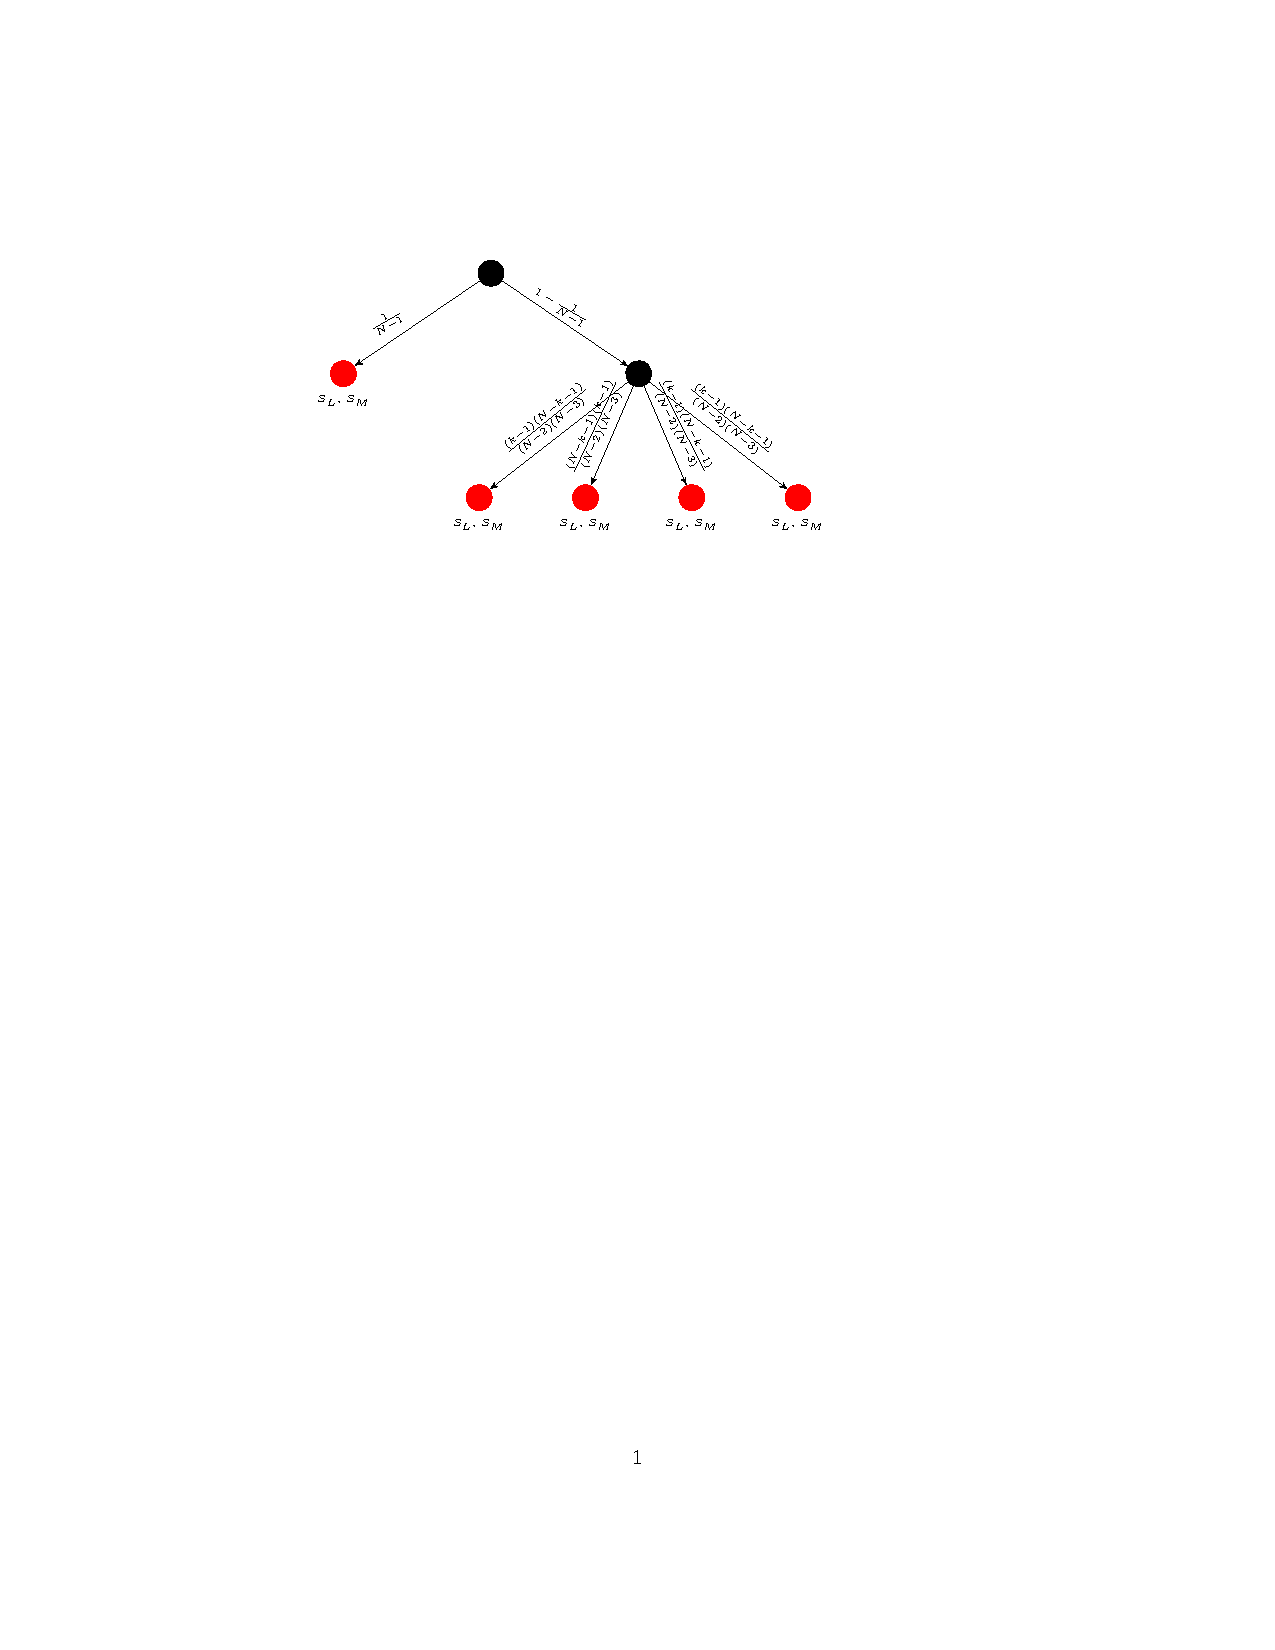
\includegraphics[width=.65\textwidth]{static/last_rounds_matches.tex}
  \caption{\textbf{Possible pairings combination in the updating stage, given
  that individuals interact with only one other member in the population.} At
  each step of the evolutionary process we choose a role model and a learner to
  update the population. We consider the case where both the role model and the
  learner estimate their fitness after interacting with a single member of the
  population. There are five possible pairings at each step. They interact with
  other with a probability \(\frac{1}{N - 1}\), and thus they do not interact
  with other with a probability \(1 - \frac{1}{N - 1}\). In the latter case,
  each of them can interact with either a mutant or a resident. Both of them
  interact with a mutant with a probability $\frac{(k-1)(k-2)}{(N-2)(N-3)}$ and
  both interact with a resident with a probability
  $\frac{(N-k-1)(N-k-2)}{(N-2)(N-3)}$. The last two possible pairings are that
  either of them interacts with a resident whilst the other interacts with a
  mutant, and this happens with a probability
  $\frac{(N-k-1)(k-1)}{(N-2)(N-3)}$.}
  \label{fig:single_pairs}
\end{figure}

Given the last round payoff and possible pair combinations for a single
interaction, we define the probability that the respective last round payoffs of
two players \(s_1, s_2\) are given by $u_1$ and $u_2$ as,

\begin{equation}\label{eq:Chi}
\setlength{\arraycolsep}{1pt}
\begin{array}{llrl}
x(u_1,u_2)	 &=&\displaystyle \frac{1}{N\!-\!1}\cdot  &v_{u_1}(s_1,s_2)\cdot 1_{(u_1,u_2)\in \mathcal{U}^2_F}\\[0.5cm]
&+	
&\displaystyle \left(1\!-\!\frac{1}{N\!-\!1}\right)  
&\left[ \frac{k\!-\!1}{N\!-\!2}\frac{k\!-\!2}{N\!-\!3} v_{u_1}(s_1,s_2) v_{u_2}(s_2,s_2) + 
 \frac{k\!-\!1}{N\!-\!2}\frac{N\!-\!k\!-\!1}{N\!-\!3} v_{u_1}(s_1,s_2) v_{u_2}(s_2,s_1)\right.\\[0.5cm]
&&&\left. +\frac{N\!-\!k\!-\!1}{N\!-\!2}\frac{k\!-\!1}{N\!-\!3} v_{u_1}(s_1,s_1) v_{u_2}(s_2,s_2) + 
 \frac{N\!-\!k\!-\!1}{N\!-\!2}\frac{N\!-\!k\!-\!2}{N\!-\!3} v_{u_1}(s_1,s_1) v_{u_2}(s_2,s_1)\right].
\end{array}
\end{equation}

The first term on the right side corresponds to the case that the learner and
the role model happened to be matched during the game stage, which happens with
probability $\frac{1}{(N\!-\!1)}$. In that case, we note that only those payoff
pairs can occur that are feasible in a direct interaction,
$\splitatcommas{(u_1,u_2)\in \mathcal{U}^2_F:=\big\{ (R,R), (S,T), (T,S), (P,P)
\big\}}$, as represented by the respective indicator function. Otherwise, if the
learner and the role model did not interact directly, we need to distinguish
four different cases, depending on whether the learner was matched with a
resident or a mutant, and depending on whether the role model was matched with a
resident or a mutant.

Given that $N\!-\!k$ players use the resident strategy
$s_{R}\!=\!(y_{R},p_{R},q_{R})$ and that the remaining $k$ players use the
mutant strategy $s_{M}\!=\!(y_{M},p_{M},q_{M})$, the probability that the number
of mutants increases by one in one step of the evolutionary process can be
written as

\begin{align}
\lambda^+_k=\frac{N\!-\!k}{N}\cdot \frac{k}{N}\cdot \sum_{u_{R},u_{M}\in\mathcal{U}} x(u_{R},u_{M})\cdot \rho(u_{R},u_{M}), \\
\lambda^-_k=\frac{N\!-\!k}{N}\cdot \frac{k}{N}\cdot \sum_{u_{R},u_{M}\in\mathcal{U}} x(u_{R},u_{M})\cdot \rho(u_{M},u_{R}).
\end{align}

In this expression, $\frac{(N\!-\!k)}{N}$ is the probability that the randomly
chosen learner is a resident, and $\frac{k}{N}$ is the probability that the role
model is a mutant. The sum corresponds to the total probability that the learner
adopts the role model's strategy over all possible payoffs $u_R$ and $u_M$ that
the two player may have received in their respective last rounds. We use
$x(u_R,u_M)$ to denote the probability that the randomly chosen resident
obtained a payoff of $u_R$ in the last round of his respective game, and that
the mutant obtained a payoff of $u_M$.

We extend our framework to consider the case where players update their
strategies based on the outcome of \textbf{the last two turns and based on their
interaction with two other members of the population}. At the stage game we
define the payoff of a reactive strategy in the last two rounds,
Proposition~\ref{proposition:last_two_rounds}.

\begin{Prop}\label{proposition:last_two_rounds} Consider a repeated game, with
  continuation probability $\delta$, between players with reactive strategies
  $s_1\!=\!(y_1, p_1, q_1$)  and $s_2\!=\!(y_2,p_2,q_2)$ respectively. Let
  $\mathcal{\tilde{U}} = \splitatcommas{\{RR, RS, RT, RP, SR, SS, ST, SP, TR,
  TS, TT, TP, PR, PS, PT, PP\}}$ denote the set of feasible payoffs in the last
  two rounds, and let \(\tilde{\mathbf{u}}\) be the corresponding payoff vector.
  Then the probability that the $s_1$ player receives the payoff $u\!\in\!
  \mathcal{\tilde{U}}$ in the very last two rounds of the game is given by,

  \begin{equation}
  \langle\mathbf{\tilde{v}}(s_1,s_2),\mathbf{\tilde{u}}\rangle, \text{ where } \mathbf{\tilde{v}} \in R^{16} \text{ is given by },
  \end{equation}
  \begin{equation}
    \mathbf{\tilde{v}}(s_1,s_2) = (1 - \delta) m_{a_1, a_2} \delta^2 \left[\mathbf{v_0}(I_4 - \delta M)^{-1}\right]_{a_1, a_2}, \quad  m_{a_1, a_2} \in M \ \forall \ a_1, a_2 \in \{1, 2, 3, 4\}.
  \end{equation}
\end{Prop}

In the updating stage we select a mutant and resident to be either the role
model or the learner. Given that they can interact with two other members of the
population there are a total of twenty four possible combinations of pairs
(Figure~\ref{fig:pissible_two_pairs}).

\begin{figure}[!htbp]
  \centering
  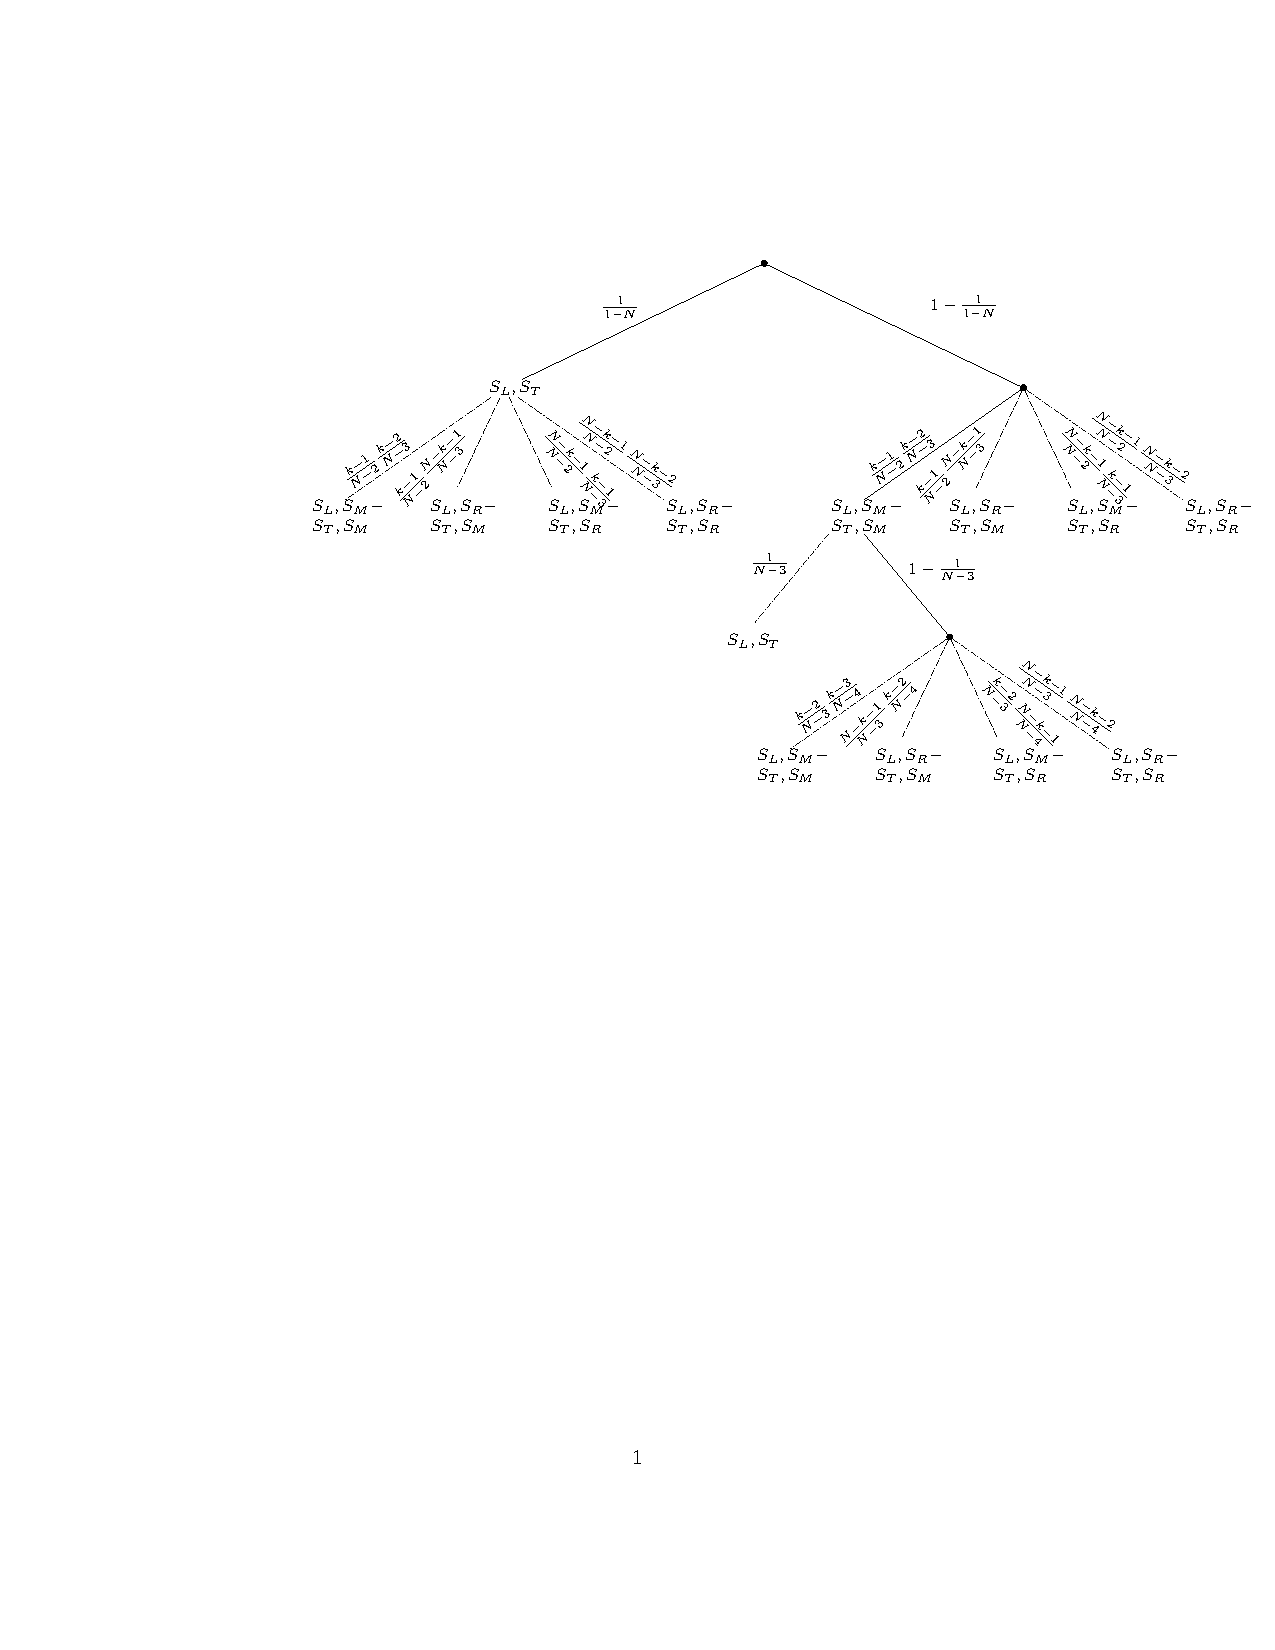
\includegraphics[width=.65\textwidth]{static/tree.tex}
  \caption{\textbf{Possible pairings combination in the updating stage, given
  that individuals interact with two other members in the population.}}
  \label{fig:pissible_two_pairs}
\end{figure}

Given the last two rounds payoff and possible pair combinations with two
members, we can define the probability \(x\) that the respective last round
payoffs of two players \(s_1, s_2\) are given by $u_1$ and $u_2$ similarly to
Eq.~(\ref{eq:Chi}). We follow the same approach to define the rest of the
updating payoffs. These are the updating payoffs of the last round with two
member, and the the last two rounds payoffs with one member.

Simulating the evolutionary process for more interactions and rounds quickly
becomes computationally intractable. Our methodology could be extended to
include \(n\) turns and \(m\) interactions. However, for the purpose of this
work we explore the cases only up to two turns and two interactions.


\section{Evolutionary dynamics under limited memory payoffs for various social
dilemmas}\label{appendix:further_simulation_results}

\begin{figure}[!htbp]
  \centering
  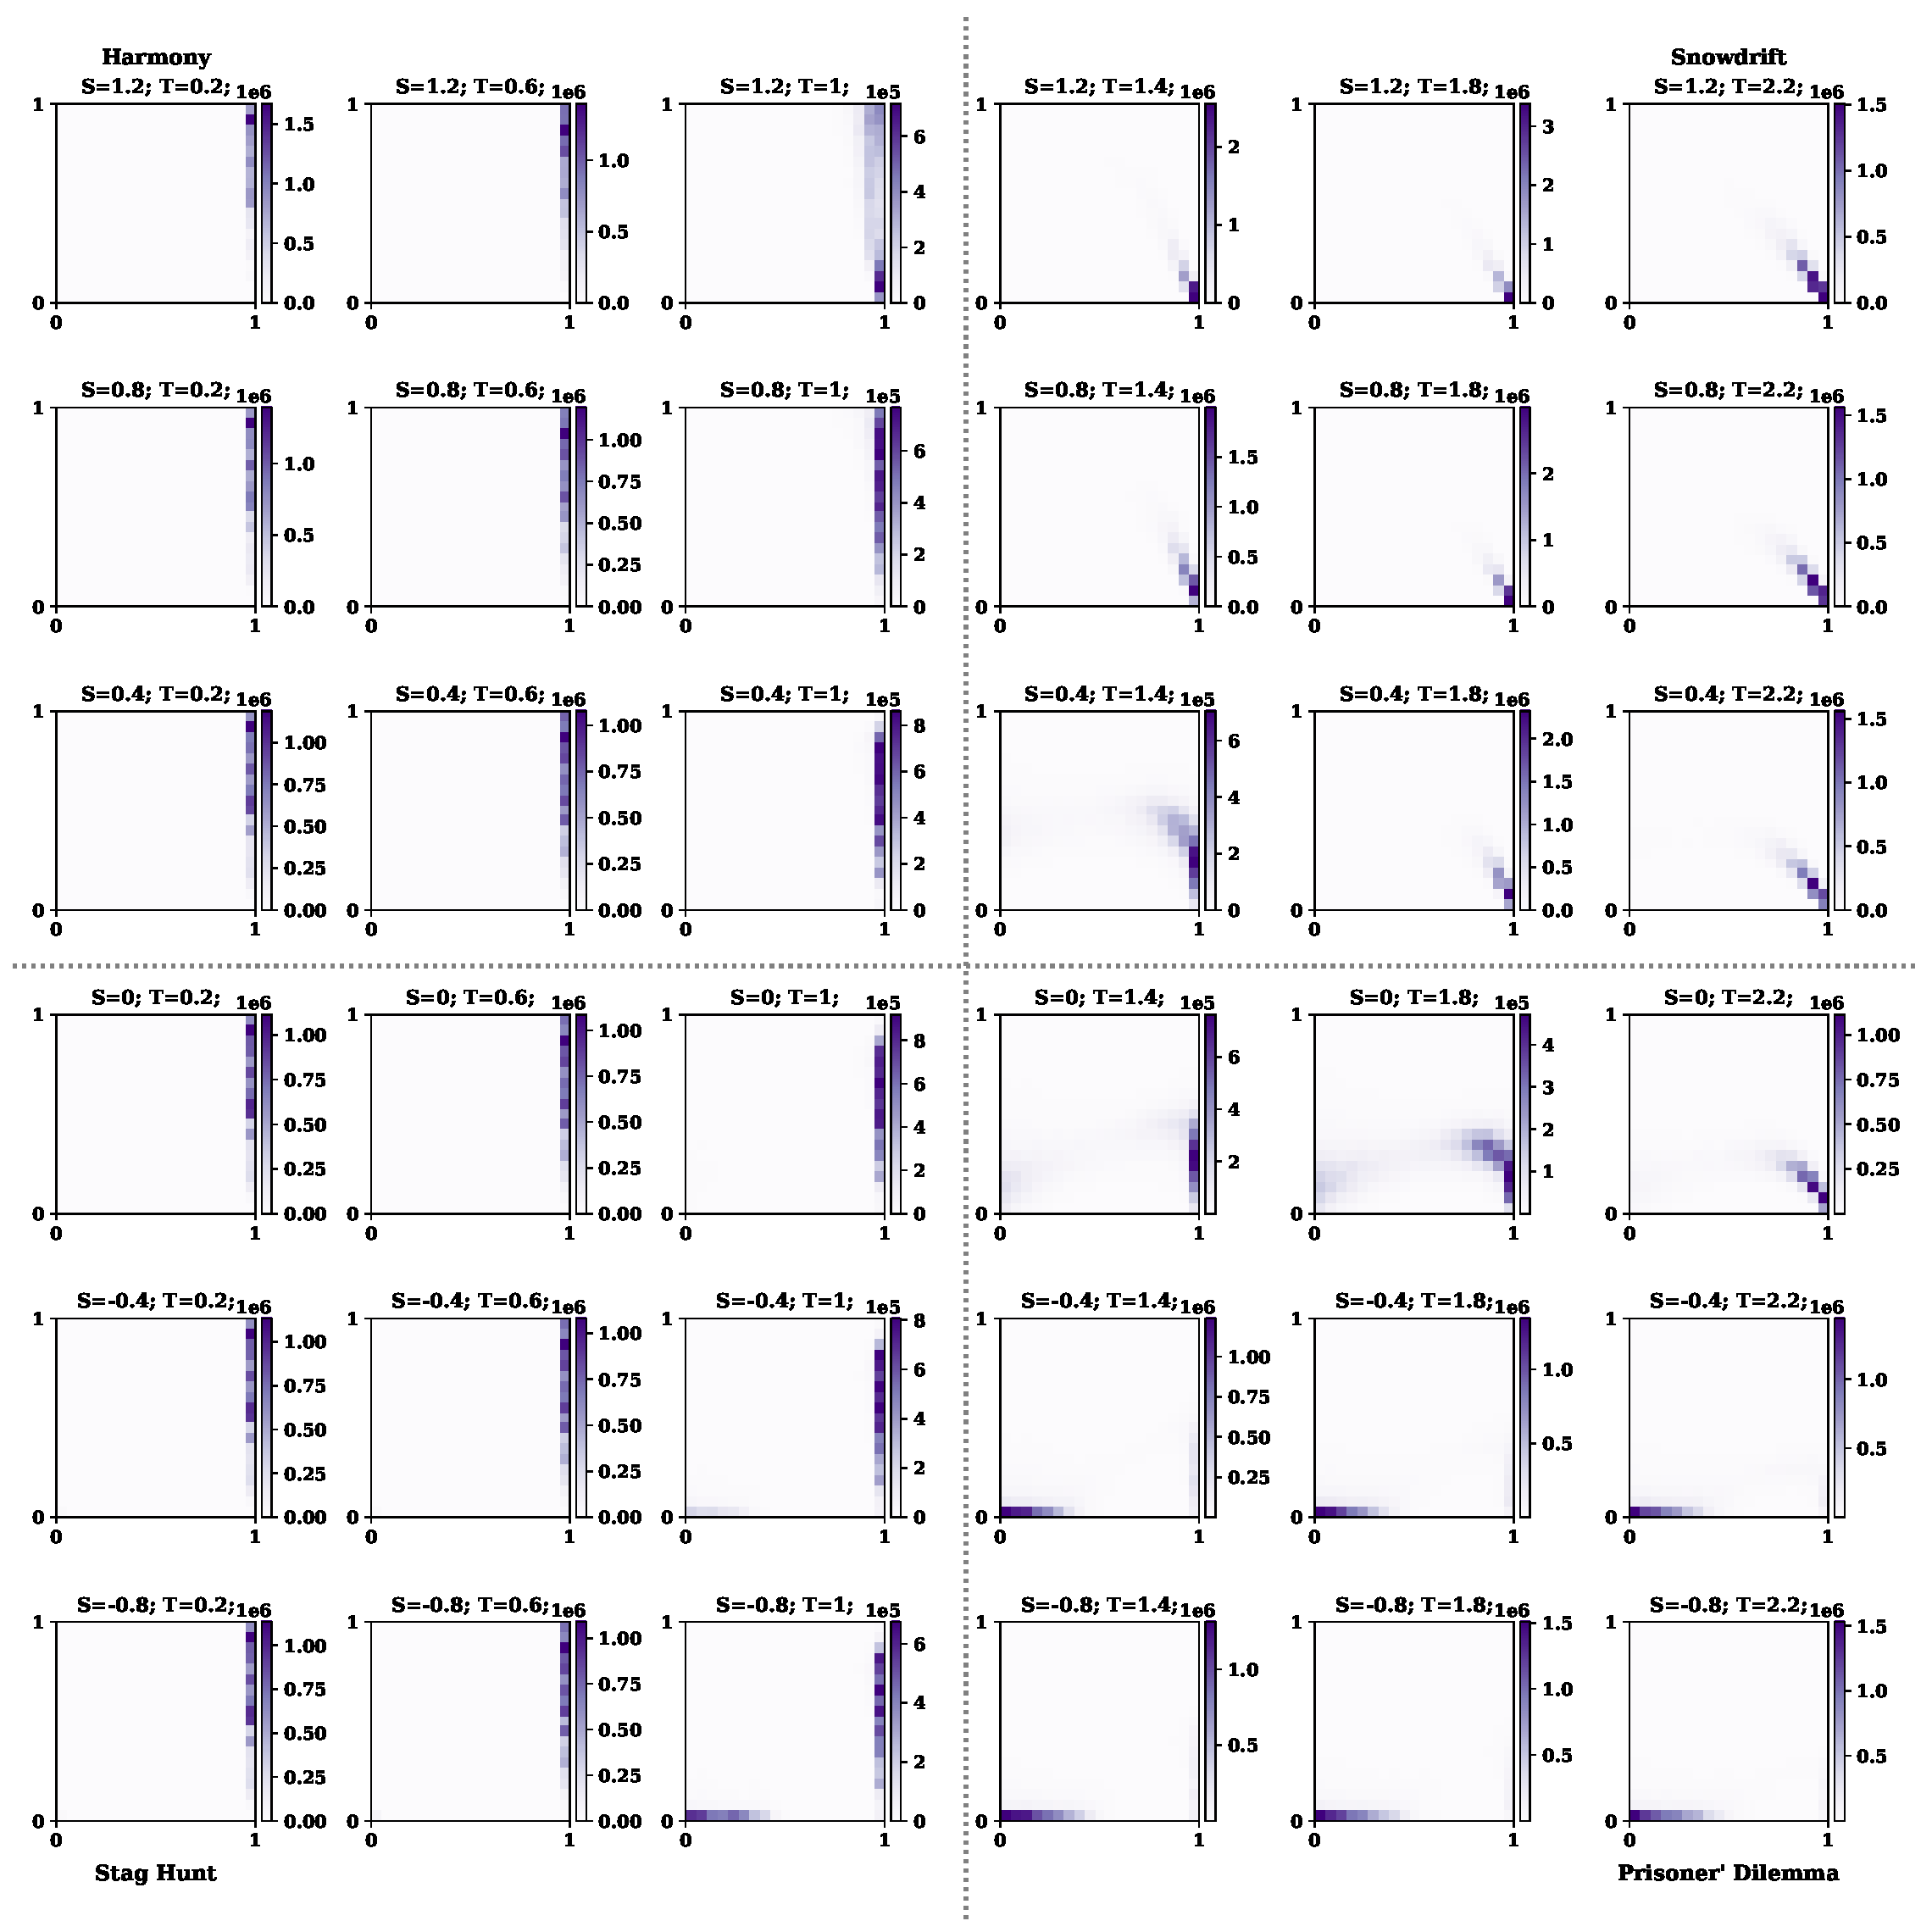
\includegraphics[width=\textwidth]{static/rounds_two_by_two_games.pdf}
  \caption{{\bf Evolutionary dynamics under last two rounds payoffs for various social dilemmas.} 
  We have run several simulations of the evolutionary process described in
  section~\ref{section:model} for $t\!=\!10^7$ time steps. The graphs show how
  often the resident population chooses each combination ($p,q$) of conditional
  cooperation probabilities in the subsequent rounds. We vary the temptation
  payoff \(T \in \{-1, -0.6, -0.2,  0.2, 0.6, 1, 1.4, 1.8, 2.2, 2.6, 3\}\)
  across the \(x\) axis, and  \(S \in \{2, 1.6, 1.2, 0.8, 0.4, 0, -0.4, -0.8,
  -1.2, -1.6, -2\}\) across the \(y\) axis. Parameters: $N\!=\!100$,
  $\beta\!=\!10$, $\delta\!=\!0.999$.}
  \label{fig:last_two_rounds_two_by_two}
\end{figure}

\begin{figure}[!htbp]
  \centering
  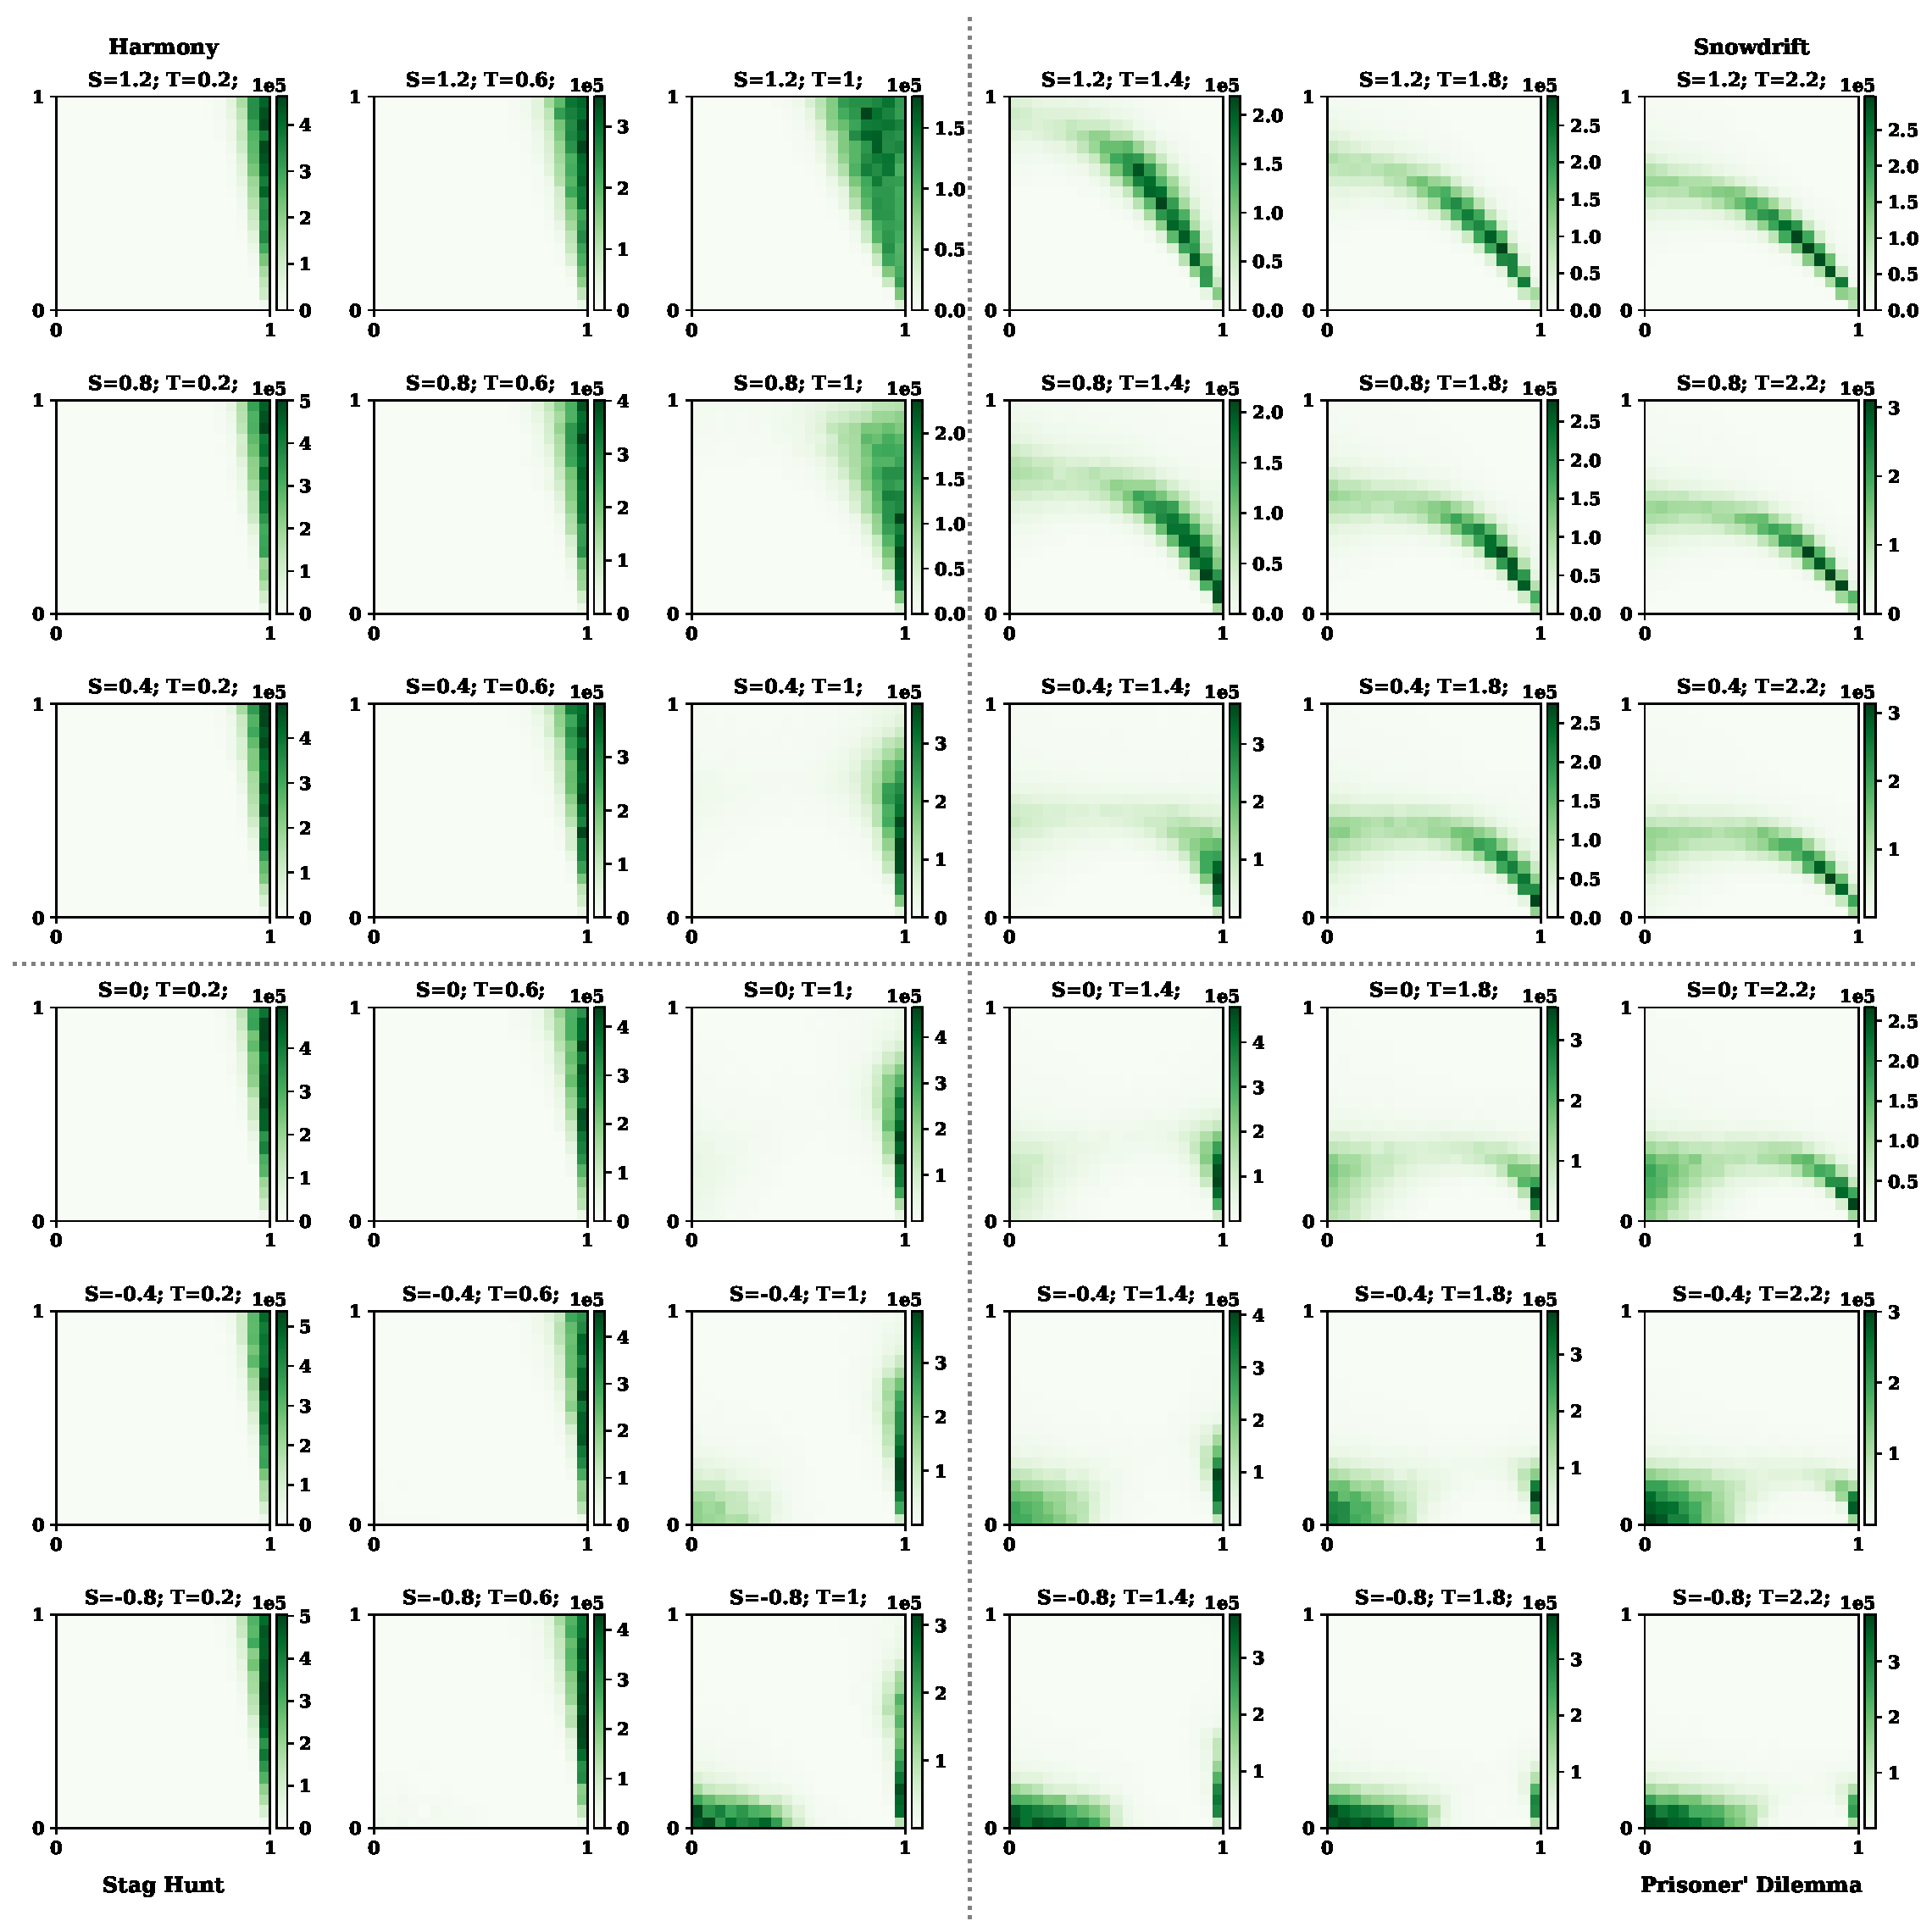
\includegraphics[width=\textwidth]{static/opponents_two_by_two_games.pdf}
  \caption{{\bf Evolutionary dynamics under last round payoffs with two members of the population for various social dilemmas.} 
  We have run several simulations of the evolutionary process described in
  section~\ref{section:model} for $t\!=\!10^7$ time steps. The graphs show how
  often the resident population chooses each combination ($p,q$) of conditional
  cooperation probabilities in the subsequent rounds. We vary the temptation
  payoff \(T \in \{-1, -0.6, -0.2,  0.2, 0.6, 1, 1.4, 1.8, 2.2, 2.6, 3\}\)
  across the \(x\) axis, and  \(S \in \{2, 1.6, 1.2, 0.8, 0.4, 0, -0.4, -0.8,
  -1.2, -1.6, -2\}\) across the \(y\) axis. Parameters: $N\!=\!100$,
  $\beta\!=\!10$, $\delta\!=\!0.999$.}
  \label{fig:last_two_opponents_two_by_two}
\end{figure}

\begin{figure}[!htbp]
  \centering
  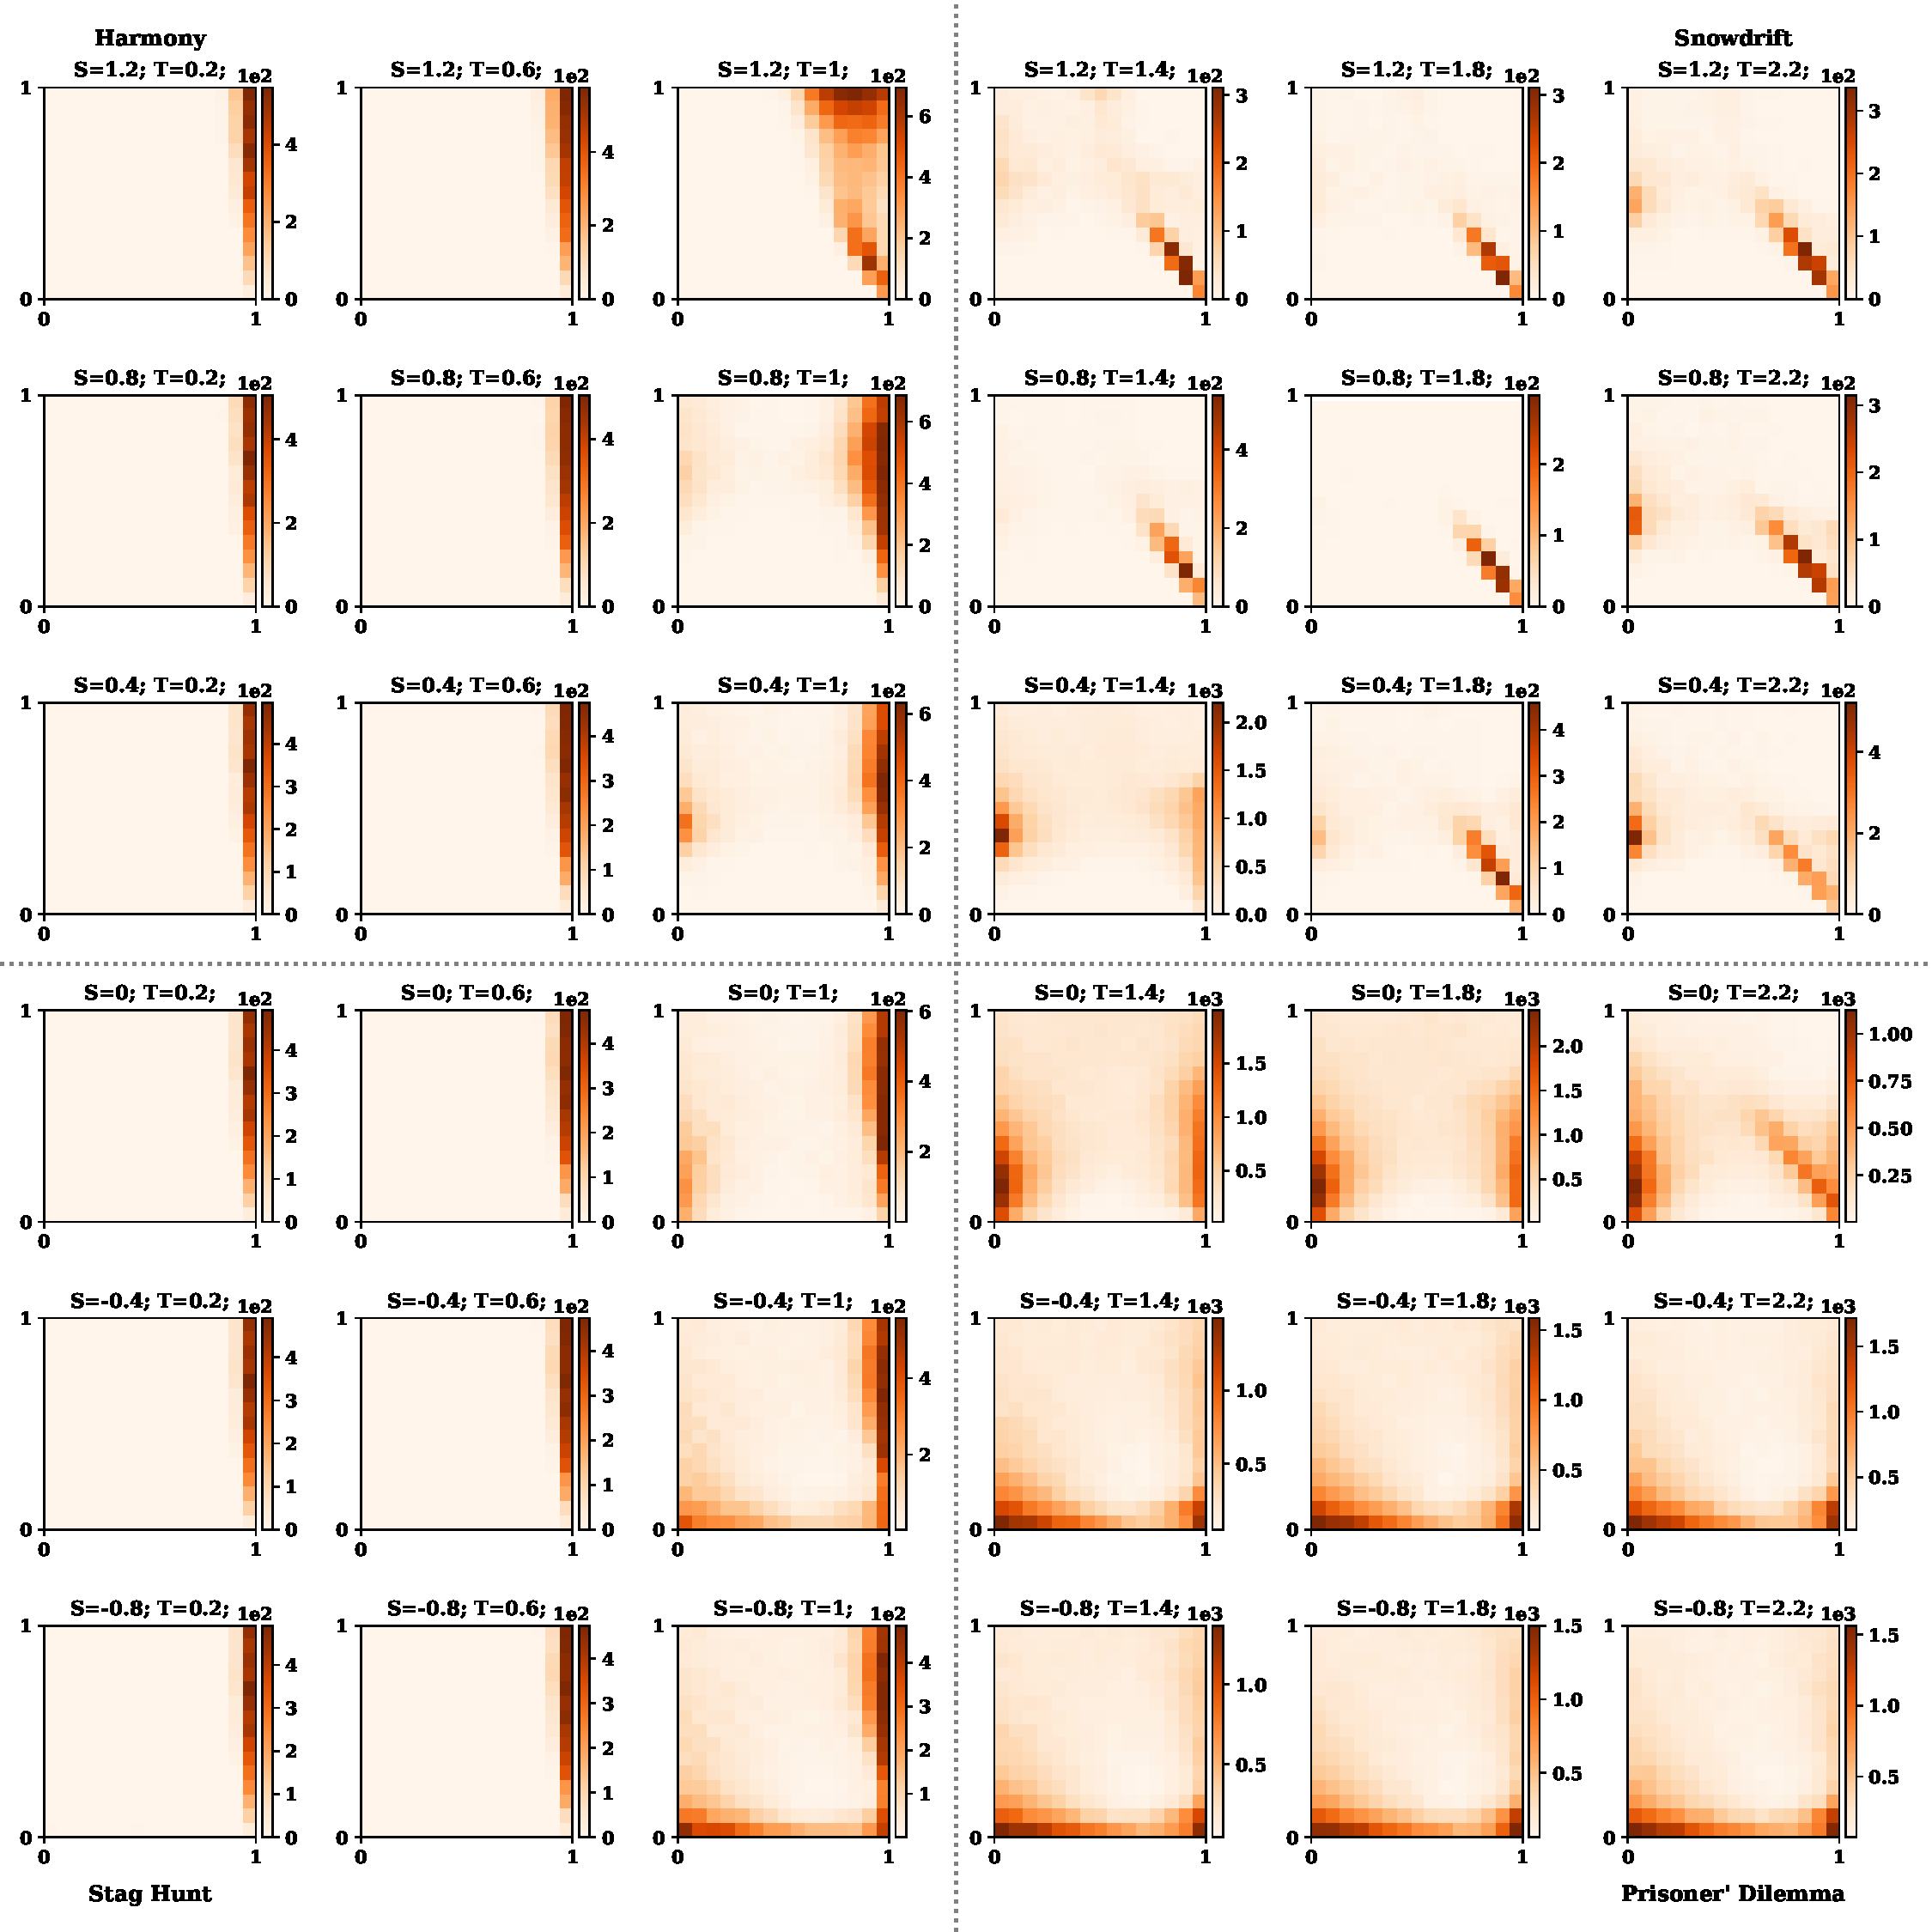
\includegraphics[width=\textwidth]{static/merged_plot_rounds_opponents_two.pdf}
  \caption{{\bf Evolutionary dynamics under last two rounds payoffs with two members of the population for various social dilemmas.} 
  We have run several simulations of the evolutionary process described in
  section~\ref{section:model} for $t\!=\!10^7$ time steps. The graphs show how
  often the resident population chooses each combination ($p,q$) of conditional
  cooperation probabilities in the subsequent rounds. We vary the temptation
  payoff \(T \in \{-1, -0.6, -0.2,  0.2, 0.6, 1, 1.4, 1.8, 2.2, 2.6, 3\}\)
  across the \(x\) axis, and  \(S \in \{2, 1.6, 1.2, 0.8, 0.4, 0, -0.4, -0.8,
  -1.2, -1.6, -2\}\) across the \(y\) axis. Parameters: $N\!=\!100$,
  $\beta\!=\!10$, $\delta\!=\!0.999$.}
  \label{fig:last_two_rounds_two_opponents}
\end{figure}

\bibliographystyle{unsrt}
\bibliography{bibliography.bib}



\end{document}
